\documentclass[12pt]{article}

% Packages nécessaires
\usepackage[T1]{fontenc}
\usepackage[utf8]{inputenc} % Encodage UTF-8 pour les caractères spéciaux
\usepackage[french,shorthands=off]{babel} % Typographie française
\usepackage{fancyhdr}
\usepackage{csquotes}
\usepackage{algorithm} % Faire des algos
\usepackage{algpseudocode}
\usepackage{caption} % Légendes pour les images
\usepackage{subcaption} % Sous-légendes
\usepackage[table]{xcolor} % Couleurs dans les tableaux
\usepackage[colorlinks=true, linkcolor=blue, citecolor=green]{hyperref}
\usepackage{tabto}
\usepackage{awesomebox}
\usepackage[left=1.5cm,right=1.5cm,top=1.75cm,bottom=2.25cm]{geometry} % Marges
\usepackage{array,mathtools} % Alignements dans les tableaux
\usepackage{parskip} % Espacement des paragraphes
\usepackage{amsmath} % Environnements mathématiques
\usepackage{graphicx} %Deja installé en principe
\usepackage{pgfplots} % Graphiques
\pgfplotsset{compat=1.18} % Définir la compatibilité sur 1.18
\usepackage{titletoc} % Pour personnaliser la table des matières
\usepackage[export]{adjustbox}
\usepackage{enumitem} % Listes personnalisées
\usepackage[backend=biber,sorting=none]{biblatex} % Bibliographie
\usepackage{amssymb} % MATHS !! (N, R, Q etc)
\setlength{\headheight}{15pt} % Hauteur des en-têtes
\setlength\bibitemsep{2\itemsep} % Espacement entre items bibliographiques
\usepackage{multirow}
\usepackage{xcolor} %\textcolor{red}{texte en rouge} OU pour un bloc : {\color{red} blabla}
% \definecolor{monbleu}{RGB}{0, 102, 204} \textcolor{monbleu}{blabla dans ma couleur bleue personnalisée}
\usepackage{float} %Pour que les conditions de figure soient plus strictes et que les graphes se placent bien au bon endroit
\usepackage{array} %Pour changer la taille de la police localement
%*{\scriptsize \setlength{\tabcolsep}{2pt} \setlength{\extrarowheight}{3pt} % Augmente l'espace de 3pt au-dessus de chaque ligne }
%\usepackage{hyperref} % tres optionnel
\usepackage{fancybox} %Pour faire des boites
\usepackage{ulem} % Pour les ... des titres (dashuline)
\usepackage{minted} 
\usepackage{forest}
\usepackage{caption}

% TikZ (déjà via pgfplots), activer des librairies utiles
\usetikzlibrary{arrows.meta,shapes.geometric,positioning}

% Styles de l’organigramme
\tikzset{
  >=Latex,
  organi/.style={font=\small, line width=0.8pt},
  startstop/.style={
    rectangle, rounded corners, minimum width=42mm, minimum height=7mm,
    draw, align=center, fill=gray!10
  },
  io/.style={
    trapezium, trapezium left angle=70, trapezium right angle=110,
    minimum width=48mm, minimum height=7mm, draw, align=center, fill=blue!5
  },
  process/.style={
    rectangle, rounded corners, minimum width=52mm, minimum height=7mm,
    draw, align=center, fill=green!5
  },
  loop/.style={
    rectangle, rounded corners, minimum width=60mm, minimum height=7mm,
    draw, align=left, fill=orange!8, dashed
  },
  dataout/.style={
    rectangle, rounded corners,
    draw, align=left, fill=purple!6, minimum width=60mm
  },
  arrow/.style={->, rounded corners=2mm}
}


\usepackage{listings} %Ecrire du CODE C
\usepackage{listingsutf8} % indispensable pour les accents dans listings (CODE !!)
\definecolor{Cbckgd}{rgb}{1,1,0.9}
\definecolor{Ckeywords}{rgb}{0.7,0,0}
\lstnewenvironment{cpp}{%
	  \lstset{
    language=[ISO]cpp,
    inputencoding=utf8,
    basicstyle=\ttfamily\fontsize{12}{14}\selectfont, % Police 12pt
    keywordstyle=\color{blue}\bfseries,               % Mots-clés en bleu gras
    identifierstyle=\color{black},                    % Identifiants en noir
    commentstyle=\color{Ccomments}\itshape,                % Commentaires en gris italique
    stringstyle=\color{teal},                         % Chaînes en vert-bleu
    numbers=left,                                     % Numérotation des lignes à gauche
    numberstyle=\tiny\color{gray},                    % Style des numéros
    numbersep=8pt,                                    % Espace entre numéro et code
    frame=single,                                     % Bordure autour du code
    rulecolor=\color{black},                          % Couleur de la bordure
    showstringspaces=false,                           % Pas d’espaces visibles dans les chaînes
    tabsize=4,                                        % Largeur des tabulations
    breaklines=true,                                  % Retour à la ligne automatique
    literate=
  {é}{{\'e}}1 {è}{{\`e}}1 {ê}{{\^e}}1 {ë}{{\"e}}1
  {à}{{\`a}}1 {â}{{\^a}}1 {ä}{{\"a}}1
  {î}{{\^i}}1 {ï}{{\"i}}1
  {ô}{{\^o}}1 {ö}{{\"o}}1
  {ù}{{\`u}}1 {û}{{\^u}}1 {ü}{{\"u}}1
  {ç}{{\c c}}1 {Ç}{{\c C}}1
  {É}{{\'E}}1 {È}{{\`E}}1 {Ê}{{\^E}}1
  {’}{{'}}1 {‘}{{'}}1 {“}{{"}}1 {”}{{"}}1
  {–}{{-}}1 {—}{{-}}1 {…}{{\ldots}}1
  {·}{{$\cdot$}}1,
    captionpos=b,                                     % Légende en bas (si utilisée)
    backgroundcolor=\color{Cbckgd}
    }}{}
    
\lstnewenvironment{C}{%
	  \lstset{
    language=C,
    inputencoding=utf8,
    basicstyle=\ttfamily\fontsize{10}{10}\selectfont, % Police 12pt
    keywordstyle=\color{Ckeywords}\bfseries,               % Mots-clés en bleu gras
    identifierstyle=\color{black},                    % Identifiants en noir
    commentstyle=\color{Ccomments}\itshape,                % Commentaires en gris italique
    stringstyle=\color{teal},                         % Chaînes en vert-bleu
    numbers=left,                                     % Numérotation des lignes à gauche
    numberstyle=\tiny\color{gray},                    % Style des numéros
    numbersep=8pt,                                    % Espace entre numéro et code
    frame=single,                                       % Bordure autour du code
    rulecolor=\color{black},                          % Couleur de la bordure
    showstringspaces=false,                           % Pas d’espaces visibles dans les chaînes
    tabsize=4,                                        % Largeur des tabulations
    breaklines=true,                                  % Retour à la ligne automatique
    literate=
  {é}{{\'e}}1 {è}{{\`e}}1 {ê}{{\^e}}1 {ë}{{\"e}}1
  {à}{{\`a}}1 {â}{{\^a}}1 {ä}{{\"a}}1
  {î}{{\^i}}1 {ï}{{\"i}}1
  {ô}{{\^o}}1 {ö}{{\"o}}1
  {ù}{{\`u}}1 {û}{{\^u}}1 {ü}{{\"u}}1
  {ç}{{\c c}}1 {Ç}{{\c C}}1
  {É}{{\'E}}1 {È}{{\`E}}1 {Ê}{{\^E}}1
  {’}{{'}}1 {‘}{{'}}1 {“}{{"}}1 {”}{{"}}1
  {–}{{-}}1 {—}{{-}}1 {…}{{\ldots}}1
  {·}{{$\cdot$}}1,
    captionpos=b,                                     % Légende en bas (si utilisée)
    backgroundcolor=\color{Cbckgd}
    }}{}


%Couleurs pour le C
\definecolor{Ckeywords}{RGB}{255,0,128}  % rose
\definecolor{Cvariables}{RGB}{0,102,204} % bleu pour les variables
\definecolor{Ccomments}{RGB}{0,128,0}    % vert pour les commentaires
\definecolor{Cstrings}{RGB}{160,32,240}  % violet pour les chaînes



% Configuration des en-têtes et pieds de page
\pagestyle{fancy}
\lhead{\textbf{LABORDE-LAULHE Alban | FABRICI Mattéo}}
\rhead{
\includegraphics[width=0.08\linewidth]{logo chimieparistech.png}}
\rfoot{\theauthor}
\renewcommand{\footrulewidth}{0.4pt}
\lfoot{\textbf{Rapport - Projet Informatique}}
\rfoot{12/10/2025}

% Définir les symboles pour chaque niveau d'indentation
\setlist[itemize,1]{label={$\bullet$}} % Premier niveau
\setlist[itemize,2]{label={$\circ$}}  % Deuxième niveau
\setlist[itemize,3]{label={--}}  % Troisième niveau

% Personnalisation de la table des matières
\titlecontents{section}[0em]{}{\bfseries\contentslabel{1.3em}}{}{\bfseries\hfill\contentspage}[\vspace{1.2ex}] 
\setcounter{tocdepth}{1} % Exclure les sous-sous-sections de la table des matières

\bibliography{name} % POUR FAIRE LE LIEN ENTRE .BIB ET .TEX
% Commandes personnalisées pour le titre
\makeatletter
\let\thetitle\@title
\let\theauthor\@author
\let\thedate\@date
\makeatother





% Titre, auteur et date
\title{\textbf{Compte Rendu}}
\author{}
\date{\textbf{\today}}

\DeclareCaptionType{extrait}[Extraits]
\begin{document}


% En-tête principale
\begin{center}
    \begin{figure}
        \centering
        
\includegraphics[width=0.2\linewidth]{logo chimieparistech.png}
        \label{fig:enter-label}
    \end{figure}
    {\LARGE{\textbf{Rapport Projet Informatique}}}\\\vspace{0.2cm}
    {\Large {Localisation d'Orbitales - FL05}}\\\vspace{0.7cm}
    \rule[1ex]{\textwidth}{0.1pt}\\
\end{center}

\tableofcontents % Décommenter pour afficher la table des matières

\section{Introduction}
%intro + description du sujet et intérêt de la programmation dans ce cas

L’étude des orbitales moléculaires constitue un outil essentiel en chimie quantique pour comprendre la structure électronique des molécules. Toutefois, les orbitales issues de la résolution de l'équation de Schrödinger sont généralement délocalisées, et cela se voit sur les représentations. Ceci les rend peu intéressante à interpréter chimiquement, notamment car elle ne représente pas les liaisons ou les doublets non liants. Pour pallier à cette difficulté, plusieurs méthodes de localisation des orbitales ont été développées. Parmi elles, l’approche POPLOC (\textit{population localised orbitals}) utilisée dans l'article est celle que nous allons suivre, apparemment la plus efficace pour notre objectif. Elle permet de transformer les orbitales délocalisées en orbitales localisées (LMO), directement interprétables en fonction des liaisons chimiques, et ce sans recourir à des calculs lourds d’intégrales biélectroniques.

Dans ce travail, nous nous intéressons à l’implémentation de cette méthode à travers un programme écrit en C. Ce programme a pour objectif de résoudre le problème posé par l’algorithme POPLOC : à partir de la matrice des coefficients d’orbitales moléculaires (E), identifier les combinaisons linéaires menant aux orbitales localisées. L’intérêt de ce développement est double. D’une part, il offre une meilleure compréhension des résultats quantiques en permettant une interprétation chimique visuelle à l'aide de logiciels tel que JMOL à partir de la nouvelle matrice des coefficients. D’autre part, il permet une automatisation, une reproductibilité et une rapidité d’exécution adaptées à l’analyse de systèmes moléculaires de complexité variable. 

Ceci dit, dans notre projet nous nous sommes penchés sur le cas de CH$_4$, une petite molécule sans doublets non liants afin de simplifier le problème. Nous avons donc uniquement quatre liaisons C-H à considérer dans notre programme.

Cependant avant de se pencher sur le programme et les résultats de celui-ci, il est important de rappeler les hypothèses utilisées. 
Tout d'abord, l’hypothèse de la combinaison linéaire des orbitales atomiques (\textit{LCAO}). Cette hypothèse suppose que les OA forment une base complète pour décrire l’état électronique de la molécule, ce qui permet d’écrire chaque OM ($\psi_{\mathrm{OM}}$) comme une combinaison linéaire d’OA ($\phi_i$). Elle rend le problème calculable via le principe variationnel : les coefficients ($c_i$) se déterminent en minimisant l’énergie sous contrainte de normalisation.
\[
\psi_{\mathrm{OM}}(\mathbf r)=\sum_{i=1}^{N} c_i\,\phi_i(\mathbf r)
\]
De plus, on utilise le fait que les OM occupées peuvent être localisées afin qu'elles correspondent à des liaisons ou des doublets, plus proches de la représentation chimique intuitive. En effet, les orbitales moléculaires \textbf{occupées} peuvent subir une transformation unitaire sans altérer la densité électronique ni l’énergie totale du système (s'explique car l’état électronique d’une molécule est représenté par un \textbf{déterminant} de Slater formé à partir des orbitales \textbf{occupées}), car elles \textbf{décrivent le même espace vectoriel}. Ce qui n'est pas le cas des vacantes car les mélanger avec des OM occupées modifierait l’espace vectoriel et donc la densité et l’énergie du système.

\begin{figure}[H]
    \centering
    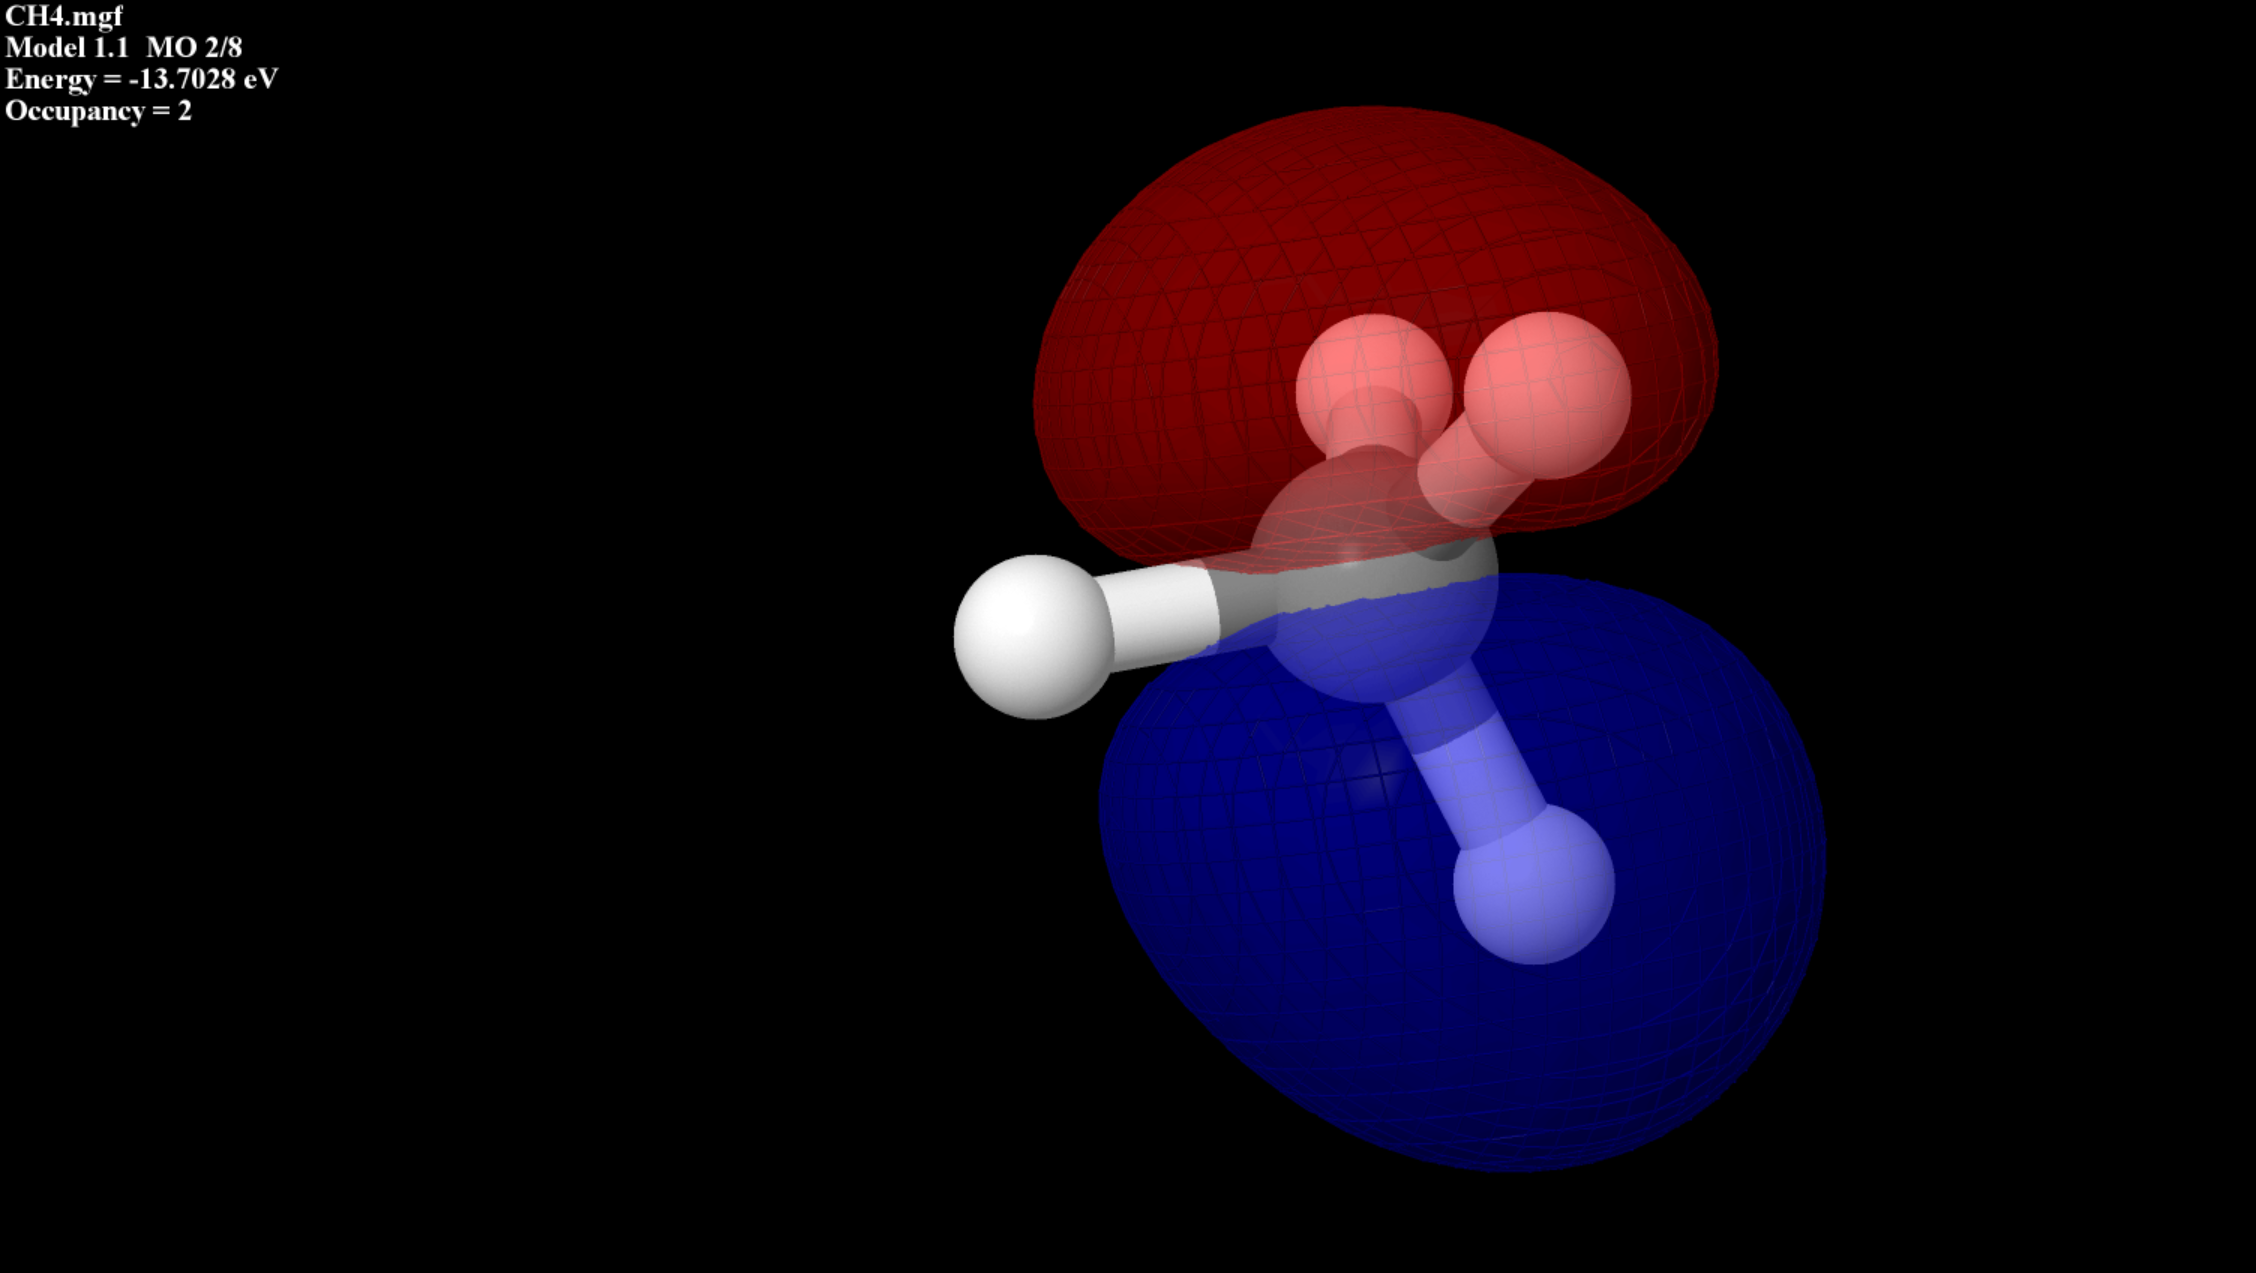
\includegraphics[width=0.45\linewidth]{images-OM/MO 2 - CH4.png}
    \caption{Exemple de représentation d'un OM délocalisée de la liaison}
    \label{fig:placeholder}
\end{figure}

\section{Méthode d'approche de l'algorithme}
%Explication de la démarche au debut pour commencer l'écriture du programme

Notre programme a pour objectif de localiser les orbitales moléculaires d'une molécule à partir d'un fichier \texttt{.mgf}  dont les orbitales sont encore délocalisées.

Pour cela, le programme doit remplir deux tâches distinctes : 
\begin{itemize}
    \item Être capable de lire et écrire un fichier \texttt{.mgf}
    \item Réaliser les opérations matricielle nécessaire à la résolution du problème.
\end{itemize}

Pour cette raison, le projet a été décomposé en 3 partie : \texttt{matrice.c} contenant l'ensemble des méthodes permettant les calculs matriciels nécessaire aux mathématiques du problème, \texttt{gestionfichier.c} contenant les méthodes pour lire et écrire un fichier \texttt{.mgf} et enfin un fichier \texttt{main.c} permettant de réaliser la localisation des orbitales grâce aux deux dépendances. 
De plus, le logiciel a besoin de deux fichiers de données : \texttt{molecule.mgf} (ici \texttt{CH4.mgf} et \texttt{liaison.csv} matrice de liaison renseignant les liaisons entre les différents atomes de la molécule.
Enfin, le programme devra retourner un fichier \texttt{.mgf} contenant les orbitales délocalisées.
L'arborescence du projet est donc la suivante : 
\begin{figure}[H]
\centering
\begin{forest}
for tree={
  font=\ttfamily,
  grow'=0,                 % arbre horizontal (racine à gauche)
  child anchor=west,
  parent anchor=east,
  anchor=west,
  l sep=40pt,               % espacement vertical entre frères
  s sep=8pt,               % espacement horizontal parent-enfant
  edge={-}                 % traits simples
}
[projet
  [src
    [main.c]
    [gestionfichier.c]
    [matrice.c]
  ]
  [includes
    [main.h]
    [gestionfichier.h]
    [matrice.h]
  ]
  [data
    [CH4.mgf]
    [liaison.csv]
  ]
  [output
    [CH4\_output.mgf]      % <-- underscore échappé
  ]
]
\end{forest}
\caption{Arborescence du projet C : structure des fichiers et répertoires.}
\label{fig:arbo}
\end{figure}

\subsection{Calcul Matriciel}

Notre programme utilise un \textit{type} personnalisée de variable appelée \texttt{Matrice} pour réaliser les calculs de la structure suivante : 

\captionof{extrait}{\texttt{includes/matrice.h}}
\begin{C}
//Définition d'une Matrice
typedef struct {
    int n;
    int m;
    long double** data;
} Matrice;
\end{C}

Ainsi, pour une matrice \texttt{Matrice M} donnée, il est possible de connaître en toute circonstance ses dimensions, via \texttt{M.n} et \texttt{M.m}. Pour lire ou écrire son contenu on utilise \texttt{M.data[i][j]} où \texttt{i} représente la ligne $i$ et \texttt{j} la colonne $j$. Cette structure nous permet de simplifier grandement les entrées et sorties des fonctions que nous utiliserons, la structure \texttt{Matrice} renseignent d'elle-même la taille de la matrice qu'elle représente simplifiant l'implémentation des calculs mathématiques. Elle permet aussi un déboggage simplifié, puisqu'il est possible de connaître à chaque étape du programme la taille des matrices utilisées.

Le fichier \texttt{matrice.h} renseigne la totalité des méthodes permettant de réaliser les opérations matricielles dont le programme a besoin mais également les méthodes pratiques d'initialisation, d'affichages et de libération d'une variable \texttt{Matrice}. Cela est décrit dans l'Extrait 2. 

\captionof{extrait}{\texttt{includes/matrice.h}}
\begin{C}[H]
//Fonctions pratiques
Matrice createMatrice(int n, int m); //Renvoie la matrice initialisée de taille n*m
void freeMatrice(Matrice *M); //Libère de la mémoire la matrice
Matrice copieMatrice(Matrice M); //Renvoie une copie dure de la Matrice M
void afficheMatrice(Matrice mat); //Affiche la matrrice dans la console
void testMatrice(Matrice M); // Transforme la matrice M en une matrice de test C(i,j) = i+j
Matrice Identite(int n); //Renvoie une Matrice identité de taille n

//Fonctions de calculs matricielles
void pScaMat(Matrice M, long double a); // a*M (sur place)
long double pScalaire(Matrice X, Matrice Y); //Produit scalaire X·Y
Matrice addMat(Matrice M, Matrice N, long double a); // M + aN
long double norme(Matrice M); //Norme d'un vecteur M
Matrice transpose(Matrice M); //Transposée de M
Matrice produit(Matrice M, Matrice N); //Produit matriciel M*N
Matrice vpDiag(Matrice D); //Vecteur des coefficients diagonaux de D
long double minVP(Matrice colVP, int *pos_out); //Valeur min et position
long double maxVP(Matrice colVP, int *pos_out); //Valeur max et position
Matrice getCol(Matrice M, int pos); //Colonne n-ième de M
int areColinear(Matrice u, Matrice v); //Colinéarité de u et v
void vpJacobi(Matrice a, Matrice b); //Jacobi: a diagonalisée, b=VP
void compareVect(Matrice u, Matrice v); // u·v / (||u||·||v||)
\end{C}

\subsection{Gestion des fichiers}
Le programme doit être capable d'ouvrir un fichier \texttt{.mgf} de le parcourir et d'en tirer les variables nécessaires au calcul. Le fichier est constitué d'une entête suivi de plusieurs ensemble de ligne correspondant à des informations sur les atomes puis les orbitales atomiques. Aucune entête ne permet de retrouver facilement chacune des sections, il est donc nécessaire de naviguer méthodiquement dans le document, en prenant en compte les informations précédemment acquise (nombre d'orbitales atomiques, nombre d'atomes) afin de sauter un nombre correct de ligne. Pour cela la méthode commence d'abord par obtenir le nombre d'atomes composant la molécule. Cela lui permet ensuite d'itérer le nombre de boucle nécessaire pour parvenir à lire l'élément chimique de chacun d'entre eux. En supposant que la molécule est exclusivement constitué de C,O,N,ou H il calcule le nombre d'orbitales atomiques dans la molécule. Cela lui permet de construire la matrice $E$, représentation des contributions des orbitales atomiques dans les orbitales moléculaires.
Au final, à partir de ce fichier le programme est capable de constituer la \texttt{Matrice E}, ainsi que le nombre d'atomes et d'électrons présent dans la molécule.

\begin{figure}[H]
  \centering
  % Losange (style de base)
\tikzset{decision/.style={diamond,aspect=2,draw,align=center,fill=red!5,inner sep=1.6pt}}
% Flèches : accroche nette aux nœuds (pas de “trous” d’1 px)
\tikzset{arrow/.style={-Latex, line width=0.6pt, shorten >=-1pt, shorten <=-1pt}}
\tikzset{organi/.style={font=\small, line width=0.6pt}}

\begin{tikzpicture}[organi, x=1cm, y=1cm]

% Rails latéraux et colonne centrale
\def\xC{0}        % centre
\def\xL{-9}       % rail gauche (branche Non de ORBITAL)
\def\xRret{ 6}    % rail droit pour le RETOUR (orbproc -> readln)
\def\xRfin{ 6.5}  % rail droit pour la FIN (EOF/Non -> close)

% ===== Colonne centrale (alignée & espacée) =====
\node[startstop]                   (start)   at (\xC,  0.0)  {Début};
\node[io,      minimum width=74mm] (in)      at (\xC, -2.6)  {Entrées : \texttt{in\_path}, \texttt{out\_path}, \texttt{E} ($nAO\times nAO$), \texttt{nAO}};
\node[process, minimum width=74mm] (open)    at (\xC, -5.4)  {Ouvrir \texttt{in} (r) et \texttt{out} (w) ; init \texttt{mo=0}};
\node[process, minimum width=74mm] (readln)  at (\xC, -8.2)  {Lire une ligne : \texttt{fgets(line,in)} ; \texttt{q = lskip(line)}};

% IF 1 : EOF ?
\node[decision,minimum width=30mm] (more)    at (\xC, -10.0) {EOF ?};

% IF 2 : ORBITAL ?
\node[decision,minimum width=30mm] (isorb)   at (\xC, -12.2) {Ligne \\ \texttt{ORBITAL} ?};

% Branche Non (à gauche) pour ORBITAL ?
\node[process, minimum width=74mm] (copyline) at (\xL, -14.4) {Recopier la ligne : \texttt{fputs(line,out)}};

% Branche Oui : traitement bloc ORBITAL (condensé)
\node[loop, minimum width=74mm] (orbproc)  at (\xC, -15.2)
  {Traiter le bloc \texttt{ORBITAL} :\\
   boucler sur \texttt{mo} lignes ; \texttt{k = count\_doubles\_in\_line} ;\\
   si \texttt{k==0} $\Rightarrow$ recopier, sinon écrire \texttt{E[got][mo]}\\ ; maj \texttt{got} ;\\
   répéter jusqu’à \(\texttt{got} = \texttt{nAO}\) ; puis \texttt{mo++}};

% Clôture
\node[startstop, minimum width=74mm] (close)    at (\xC, -18.5) {Fermer \texttt{in} et \texttt{out} ; \texttt{return 0}};

% ===== Liaisons (orthogonales, sur ancres) =====
\draw[arrow] (start.south) -- (in.north);
\draw[arrow] (in.south)    -- (open.north);
\draw[arrow] (open.south)  -- (readln.north);

% IF "EOF ?"
\draw[arrow] (readln.south) -- (more.north);
% Oui -> continuer : mini-stub + label collé, puis ORBITAL ?
\draw[arrow] (more.south) -- ++(0,-1mm) node[near start,right,yshift=-5pt]{Oui} -- (isorb.north);
% Non -> fin : mini-stub + label collé, puis rail FIN distinct jusqu’à close
\draw[arrow]
  (more.east) -- ++(9mm,0) node[near start,above]{Non}
  -- (\xRfin, -10.0)
  -- (\xRfin, -19.6 +2.5)
  -- (\xC,    -19.6 +2.5) % coude horizontal pour éviter la diagonale
  -- (close.north);
% IF "ORBITAL ?"
% Non : vers rail gauche puis bloc copyline (label collé)
\draw[arrow] (isorb.west) -- ++(-9mm,0) node[near start,above]{Non}
  -- (\xL + 1, -12.2) -- ([xshift=10mm]copyline.north);
% Oui : direct vers orbproc (label collé)
\draw[arrow] (isorb.south) -- ++(0,-1mm) node[near start,right,yshift=-5pt]{Oui} -- (orbproc.north);

% Retour Non (copie) : remonte proprement vers la lecture suivante
\draw[arrow] ([xshift=-10mm]copyline.north) |- (readln.west);

% Après traitement d'un bloc : rail RETOUR (distinct) -> readln
\draw[arrow] (orbproc.east) -- (\xRret, -15.2) |- (readln.east);

\end{tikzpicture}

  \caption{Organigramme vertical de \texttt{ecrireMGF(...)} — réécriture des blocs \texttt{ORBITAL} depuis \texttt{E}.}
  \label{fig:ecrireMGF_flowchart}
\end{figure}

\begin{figure}[H]
  \centering
  \begin{tikzpicture}[organi, node distance=8mm and 14mm]
\tikzset{organi/.style={font=\small, line width=0.6pt}}
% 1 : Début
\node[startstop] (start) {Début};

% 2 : Entrées
\node[io, below=8mm of start] (in) {Entrées : \texttt{path}, \texttt{*E}, \texttt{**aoParAtome}, \texttt{*natoms\_out}, \texttt{*ev\_out}};
\draw[arrow] (start) -- (in);

% 3 : Ouvrir fichier
\node[process, below=8mm of in] (open) {Ouvrir le fichier \\ \texttt{f = fopen(path,"r")}};
\draw[arrow] (in) -- (open);

% 4 : Lire natoms
\node[process, below=8mm of open] (readn) {Lire le nombre d'atomes $\rightarrow$ \textbf{\texttt{natoms}}};
\draw[arrow] (open) -- (readn);

% 5 : Allouer
\node[process, below=8mm of readn] (alloc) {Allouer \textbf{\texttt{aoParAtome[natoms]}} si demandé};
\draw[arrow] (readn) -- (alloc);

% 6 : Boucle atomes
\node[loop, below=8mm of alloc] (loopatoms) {Boucle $i = 1..$ \texttt{natoms} :\\
Lire $Z$, déterminer le nombre d'AO,\\
remplir \texttt{aoParAtome[i]}, cumuler $\rightarrow$ \textbf{\texttt{nAO}}};
\draw[arrow] (alloc) -- (loopatoms);

% 7 : Créer matrices
\node[process, below=8mm of loopatoms] (createE) {Créer \textbf{\texttt{E}} (\texttt{nAO$\times$nAO}) et \textbf{\texttt{ev\_out}} (\texttt{nAO$\times$1})};
\draw[arrow] (loopatoms) -- (createE);

% 8 : Boucle ORBITAL
\node[loop, below=8mm of createE] (looporb) {Boucle sur les lignes \texttt{ORBITAL} :\\
extraire énergie $\rightarrow$ \textbf{\texttt{ev\_out[i]}} ;\\
lire \texttt{nAO} coefficients $\rightarrow$ remplir la colonne $i$ de \texttt{E};\\
incrémenter $i$, compter \texttt{ORBITAL}};
\draw[arrow] (createE) -- (looporb);

% 9 : Sorties
\node[dataout, below=8mm of looporb] (outs) {\textbf{Sorties :}\\
\texttt{*E} : coefficients OA$\rightarrow$OM\\
\texttt{*ev\_out} : énergies des OM (eV)\\
\texttt{**aoParAtome} : nb d’AO par atome\\
\texttt{*natoms\_out = natoms}\\
compteur \texttt{ORBITAL}};
\draw[arrow] (looporb) -- (outs);

% 10 : Fin
\node[startstop, below=8mm of outs] (end) {Fin \& \texttt{return 1}};
\draw[arrow] (outs) -- (end);

\end{tikzpicture}



  \caption{Organigramme vertical de \texttt{lireMGF(...)}.}
  \label{fig:lireMGF_flowchart}
\end{figure}



Afin de constituer la matrice R, le programme doit également être au fait de la répartition des liaisons dans la molécule. Pour cela nous avons crée un fichier CSV représentant la matrice du graphe des liaisons présentes dans la molécule.
La fonction \texttt{lireCSV(...)} permet de récupérer cette matrice à partir du fichier CSV.

Enfin, le programme doit être capable de rédiger un fichier \texttt{.mgf} neuf (appelé ici \texttt{out.mgf}) contenant les orbitales moléculaires localisées calculées. Pour cela, il utilise comme base un fichier \texttt{.mgf} d'entrée(qu'on appelera \texttt{in.mgf})qui est celui utilisé précédemment pour acquérir les valeurs des orbitales moléculaires délocalisées. La méthode se contente de recopier identiquement ligne par ligne le fichier \texttt{in.mgf} a moins que la ligne lu commence par la chaine \texttt{"ORBITAL"}. Dans ce cas, le programme rédige une ligne correspondant aux nouveaux coefficients calculés. Enfin, la méthode termine lorqu'elle parviens à la fin du document.


\section{Organigramme \& Détail des fonctions}
%organigramme de fonctionnement du programme sur une page, puis sur les pages suivantes détails des fonctions principales en quelques lignes: prototype, description des entrées et des sorties et rôle dans le programme

\subsection{Organigramme}

\begin{figure}[H]
    \centering
    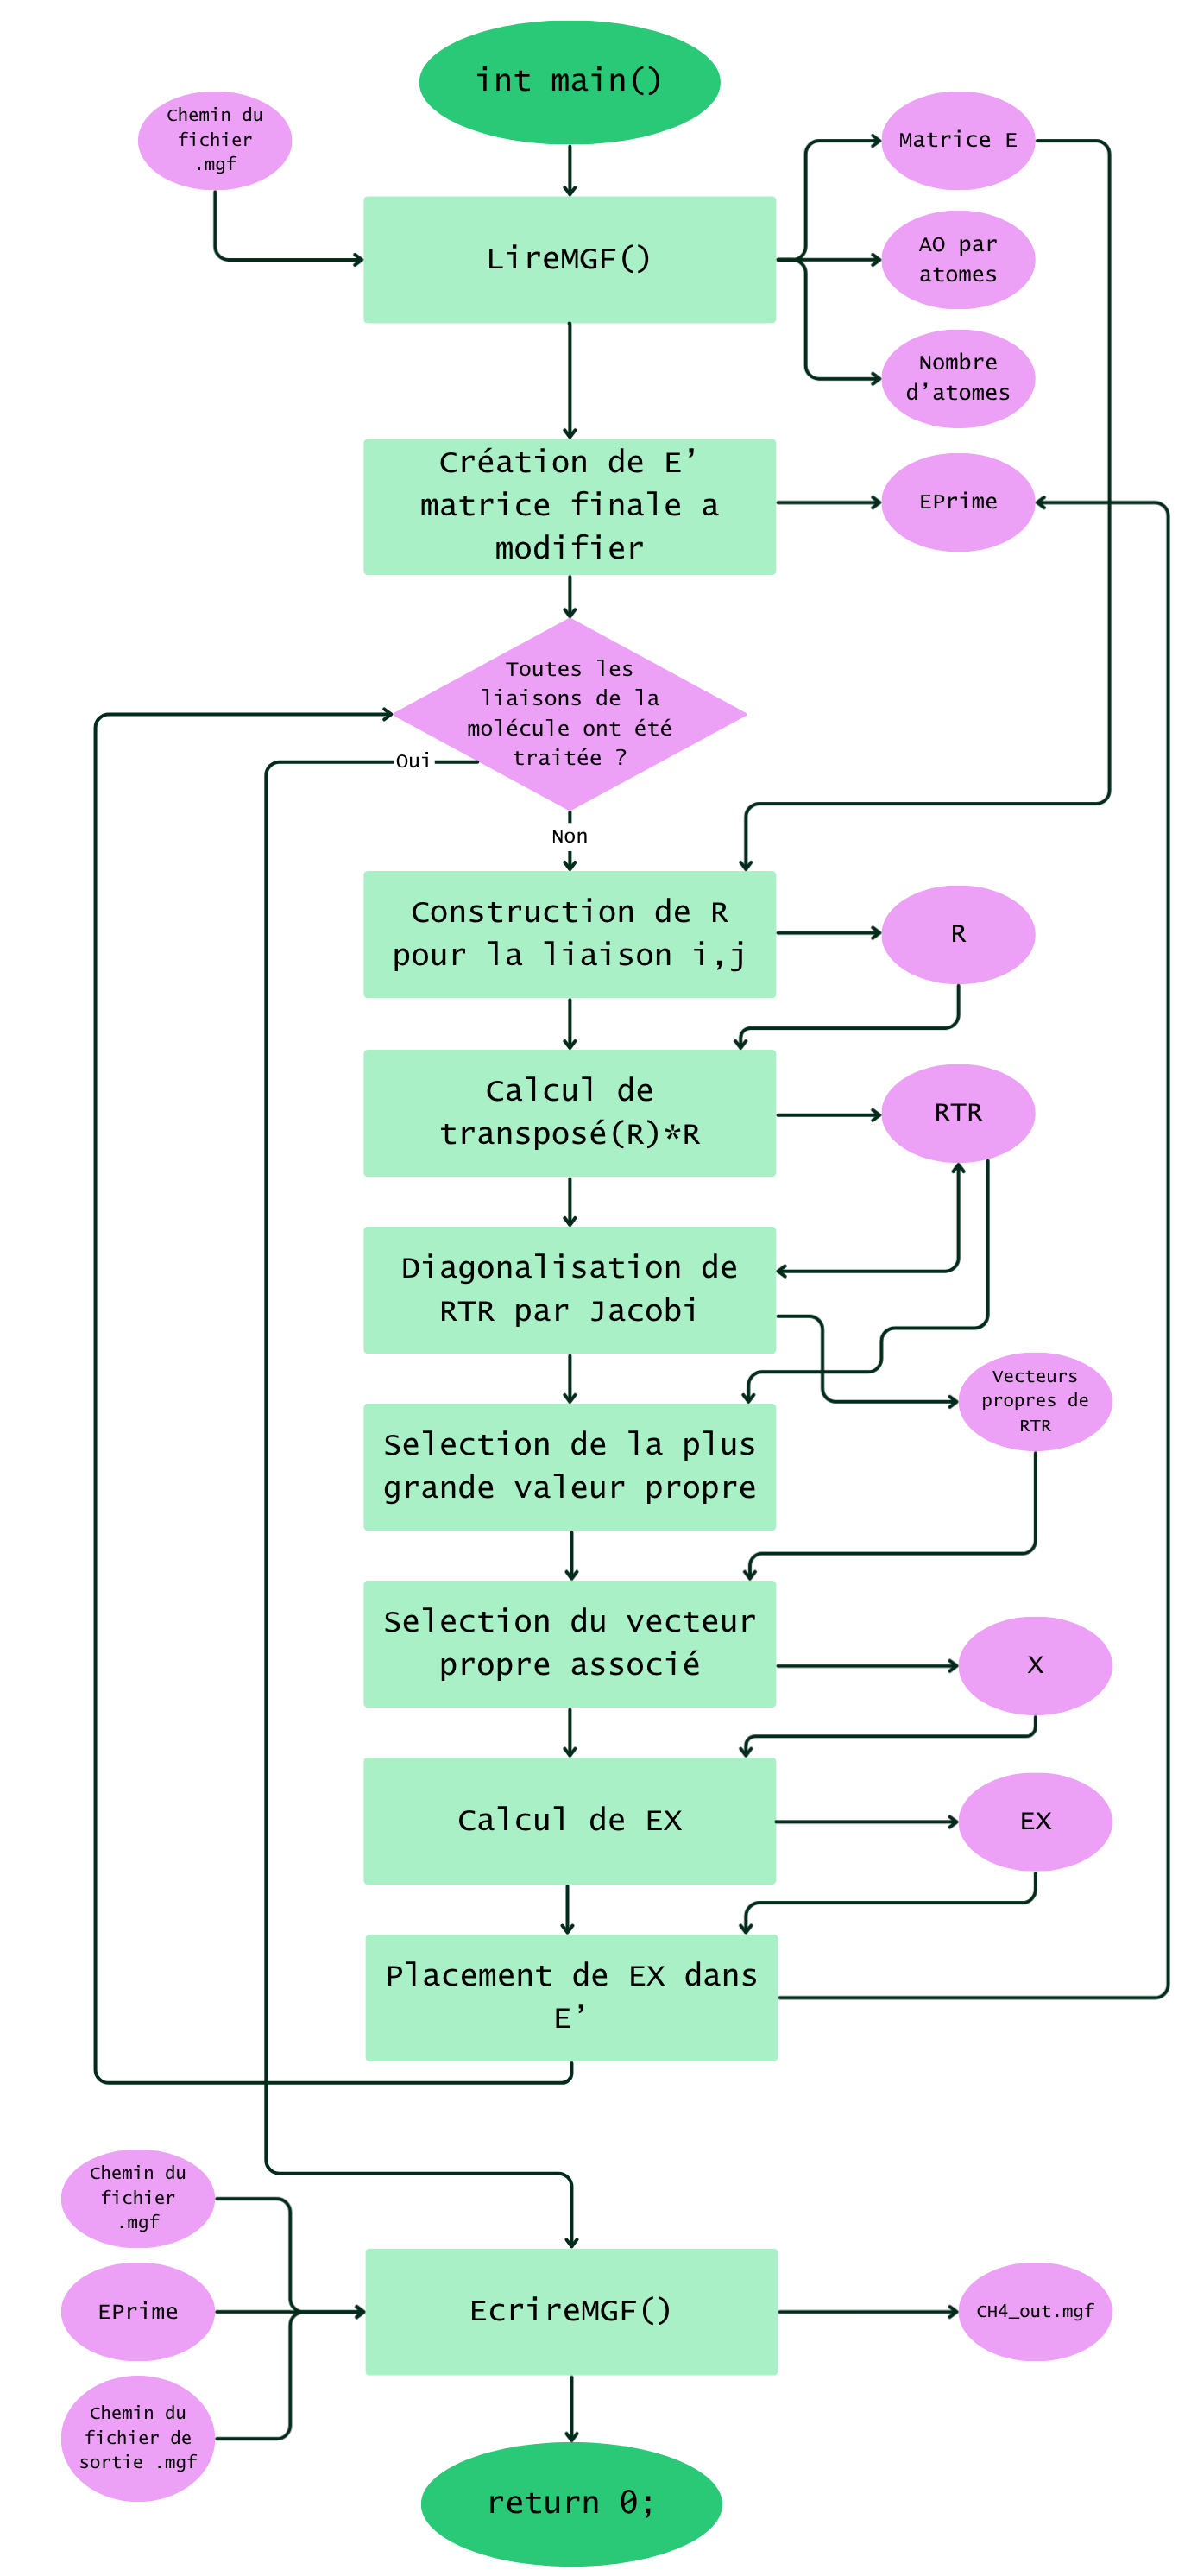
\includegraphics[width=0.51\linewidth]{images autres/Organigramme - Projet Info.png}
    \caption{Organigramme du Code}
  \label{fig:placeholder}
\end{figure}

L'objectif du programme est, à partir d'une matrice $E_{[OA][OM]}$ récupérée à partir un fichier \texttt{.mgf} de constituer une matrice des orbitales localisées $E'_{[OA][OM]}$.

En prenant l'exemple du méthane, la matrice $E$ aura l'allure suivante.

\[
E[\mathrm{OA}][\mathrm{OM}] =
\begin{bmatrix}
p_{11} & p_{12} & p_{13} & p_{14} & p_{15} & p_{16} & p_{17} & p_{18} \\
p_{21} & p_{22} & p_{23} & p_{24} & p_{25} & p_{26} & p_{27} & p_{28} \\
p_{31} & p_{32} & p_{33} & p_{34} & p_{35} & p_{36} & p_{37} & p_{38} \\
p_{41} & p_{42} & p_{43} & p_{44} & p_{45} & p_{46} & p_{47} & p_{48} \\
p_{51} & p_{52} & p_{53} & p_{54} & p_{55} & p_{56} & p_{57} & p_{58} \\
p_{61} & p_{62} & p_{63} & p_{64} & p_{65} & p_{66} & p_{67} & p_{68} \\
p_{71} & p_{72} & p_{73} & p_{74} & p_{75} & p_{76} & p_{77} & p_{78} \\
p_{81} & p_{82} & p_{83} & p_{84} & p_{85} & p_{86} & p_{87} & p_{88}
\end{bmatrix}
\]

À partir de celle-ci, on peut construire, pour chaque liaison C--H, un sous-ensemble d’orbitales locales en supprimant les lignes correspondant aux orbitales atomiques (OA) situées sur les deux atomes concernés.  
On obtient ainsi une matrice 
\[
R = P_{\mathcal{N}} E,
\]
où \(P_{\mathcal{N}}\) est le projecteur qui conserve uniquement les OA dites \emph{locales}.  
Physiquement, cela revient à isoler la contribution des orbitales moléculaires occupées par des électrons : la matrice \(R\) mesure la \emph{population électronique} des orbitales délocalisées dans la région où l’on cherche à localiser la densité électronique.

Comme l’espace engendré par les orbitales occupées est invariant par rotation unitaire, il est légitime de chercher, dans cet espace, la combinaison linéaire \(X\) qui maximise cette population non locale, c’est-à-dire le vecteur propre associé à la plus grande valeur propre de la matrice symétrique positive 
\[
R^{\mathrm T} R.
\]
La colonne correspondante 
\[
L = E X
\]
représente alors l’orbitale la plus confinée sur la liaison considérée, et l’ensemble des vecteurs propres ainsi obtenus pour les quatre liaisons C--H définit la matrice transformée 
\[
E' = E \,\widetilde{X},
\]
dont les colonnes constituent les orbitales localisées du méthane.

\subsection{Fonctions principales}


En ce qui concerne les fonctions centrales de notre programme, nous allons les détailler dans la suite :

\dashuline{Fonction \texttt{LireMGF} (cf Figure \ref{fig:lireMGF_flowchart}) :}

\begin{itemize}
    \item Prototype : 
    \begin{minted}{cpp}
int lireMGF(const char *path, Matrice *E, int **aoParAtome, int *natoms_out);
    \end{minted}
    \item Entrée : Le fichier, une matrice, un pointeur vers un tableau contenant le nombre d'Orbitales atomiques (OA) qu'un atome possède et un pointeur entier pour le nombre d'atomes de la molécule.
    \item Sortie : Renvoie une matrice E contenant les 8 orbitales moléculaires (OM) sur les colonnes en fonction des 8 OA sur les lignes. Renseigne dans les pointeurs idoines le nombre d'atomes et d'orbitales atomiques dans la molécule.
    \item Rôle : Cette fonction lit le fichier \texttt{CH4.mgf} et extrait les données des orbitales moléculaires (ici 8 mais fonctionne pour toutes les molécules de base [contenant O,N,C,H]) puis les renvoie sous forme de matrice (E).
\end{itemize}

\dashuline{Fonction \texttt{EcrireMGF} :}

\begin{itemize}
    \item Prototype : 
    \begin{minted}{cpp}
int ecrireMGF(const char *in_path, const char *out_path,const Matrice *E, int nAO);
    \end{minted}
    \item Entrée : Le chemin vers le fichier MGF a modifier, le chemin vers le nouveau fichier MGF qui va sera crée, la  matrice calculée contenant les nouveaux coefficients, le nombre d'OA de la molécule.
    \item Sortie : Modifie le fichier, renvoie 0 si le fichier a bien été modifié.
    \item Rôle : Cette fonction lit le fichier \texttt{CH4.mgf} et remplace les coefficients des OM du fichier par les nouveaux coefficients à l'aide de la nouvelle matrice E' (pour CH$_4$, les 4 nouvelles colonnes de L' et les 4 autres colonnes de E).
\end{itemize}

\dashuline{Fonction Jacobi :}

\begin{itemize}
    \item Prototype : 
    \begin{minted}{cpp}
void vpJacobi(Matrice a, Matrice b);
    \end{minted}
    \item Entrée : a = matrice carré \textbf{symétrique réelle}; \texttt{b = vecteur}.
    \item Sortie : Diagonalise la matrice \texttt{a}; \texttt{b} devient la matrice des vecteurs propres.
    \item Rôle : Elle permet de donner la \textbf{matrice des vecteurs propres} et \textbf{leurs valeurs propres associées}, indispensable pour la résolution du problème.
\end{itemize}

\dashuline{Fonction \texttt{maxVP} :}

\begin{itemize}
    \item Prototype : 
    \begin{minted}{cpp}
double maxVP(Matrice colVP, int *pos_out);
    \end{minted}
    \item Entrée : une matrice vecteur colonne, un pointeur vers un entier.
    \item Sortie : min = la valeur de la plus petite valeur propre. \texttt{pos\_out} correspond désormais à la position de cette valeur propre.
    \item Rôle : renvoie la plus petite valeur propre (min) sa position dans la matrice.
\end{itemize}

%\dashuline{Fonction pScalaire :}
    
%\begin{itemize}
%    \item Prototype : 
%    \begin{minted}{cpp}
%double pScalaire(Matrice X, Matrice Y);
%    \end{minted}
%    \item Entrée : un vecteur colonne X, un vecteur colonne Y 
%    \item Sortie : la valeur du produit scalaire 
%    \item Rôle : renvoie le produit scalaire à l'aide de la fonction produit (qui fonctionne aussi pour les matrices en général). Cette fonction est nécessaire pour la normalisation des vecteurs colonnes. 
%\end{itemize}


\dashuline{Fonction CreateMatrice :}

\begin{itemize}
    \item Prototype : 
    \begin{minted}{cpp}
Matrice createMatrice(int n, int m);
    \end{minted}
    \item Entrée : n = entier des lignes; m = entier des colonnes. 
    \item Sortie : matrice remplie de zeros de taille n*m.
    \item Rôle : Crée des matrices de taille n*m indispensables pour le problème et utilisée très souvent.
\end{itemize}

\dashuline{Fonction FreeMatrice :}

\begin{itemize}
    \item Prototype : 
    \begin{minted}{cpp}
void freeMatrice(Matrice *M);
    \end{minted}
    \item Entrée : une matrice M.
    \item Sortie : Rien.
    \item Rôle : Permet de supprimer l'espace alloué par la fonction "malloc" (utilisée dans la fonction "CreateMatrice") pour une matrice. Puisque meme si la matrice n'est plus utile, ou que le programme crash, l'espace reste alloué et cela permet de le libérer.
\end{itemize}

\dashuline{Fonction vpDiag :}

\begin{itemize}
    \item Prototype : 
    \begin{minted}{cpp}
Matrice vpDiag(Matrice D); 
    \end{minted}
    \item Entrée : une matrice Diagonale (D).
    \item Sortie : un vecteur colonne (res).
    \item Rôle : Donne un vecteur colonne des valeurs propres d'une matrice diagonale.
\end{itemize}

\dashuline{Fonction GetCol :}

\begin{itemize}
    \item Prototype : 
    \begin{minted}{cpp}
Matrice getCol(Matrice M, int pos);
    \end{minted}
    \item Entrée : une matrice M, un entier (pos) indiquant la colonne a extraire.
    \item Sortie : un vecteur colonne (res).
    \item Rôle : Permet de récupérer la colonne d'une matrice sous la forme d'un nouveau vecteur colonne à partir de son indice dans cette matrice.
\end{itemize}


\section{Résultats \& Analyse}

A la fin de l'exécution du fichier "main.c", le programme écrit un fichier "CH4\_output.mgf" (dans le dossier "output") en reprenant exactement le même formalisme que dans le fichier d'entrée "CH4.mgf". Finalement, seules les valeurs des coefficients des OA pour les OM concernées changent.
C'est-à-dire que pour le cas de CH$_4$, seules les 4 premières OM occupées vont avoir leurs coefficients modifiés (puisqu'il y a 8 électrons de valence mis en jeu). On visualise donc via le logiciel Jmol les 4 nouvelles OM ainsi que les anciennes afin de les comparer. Afin de mieux visualiser les lobes, 

\begin{figure}[H]
    \centering
    \begin{subfigure}{0.48\textwidth}
        \centering
        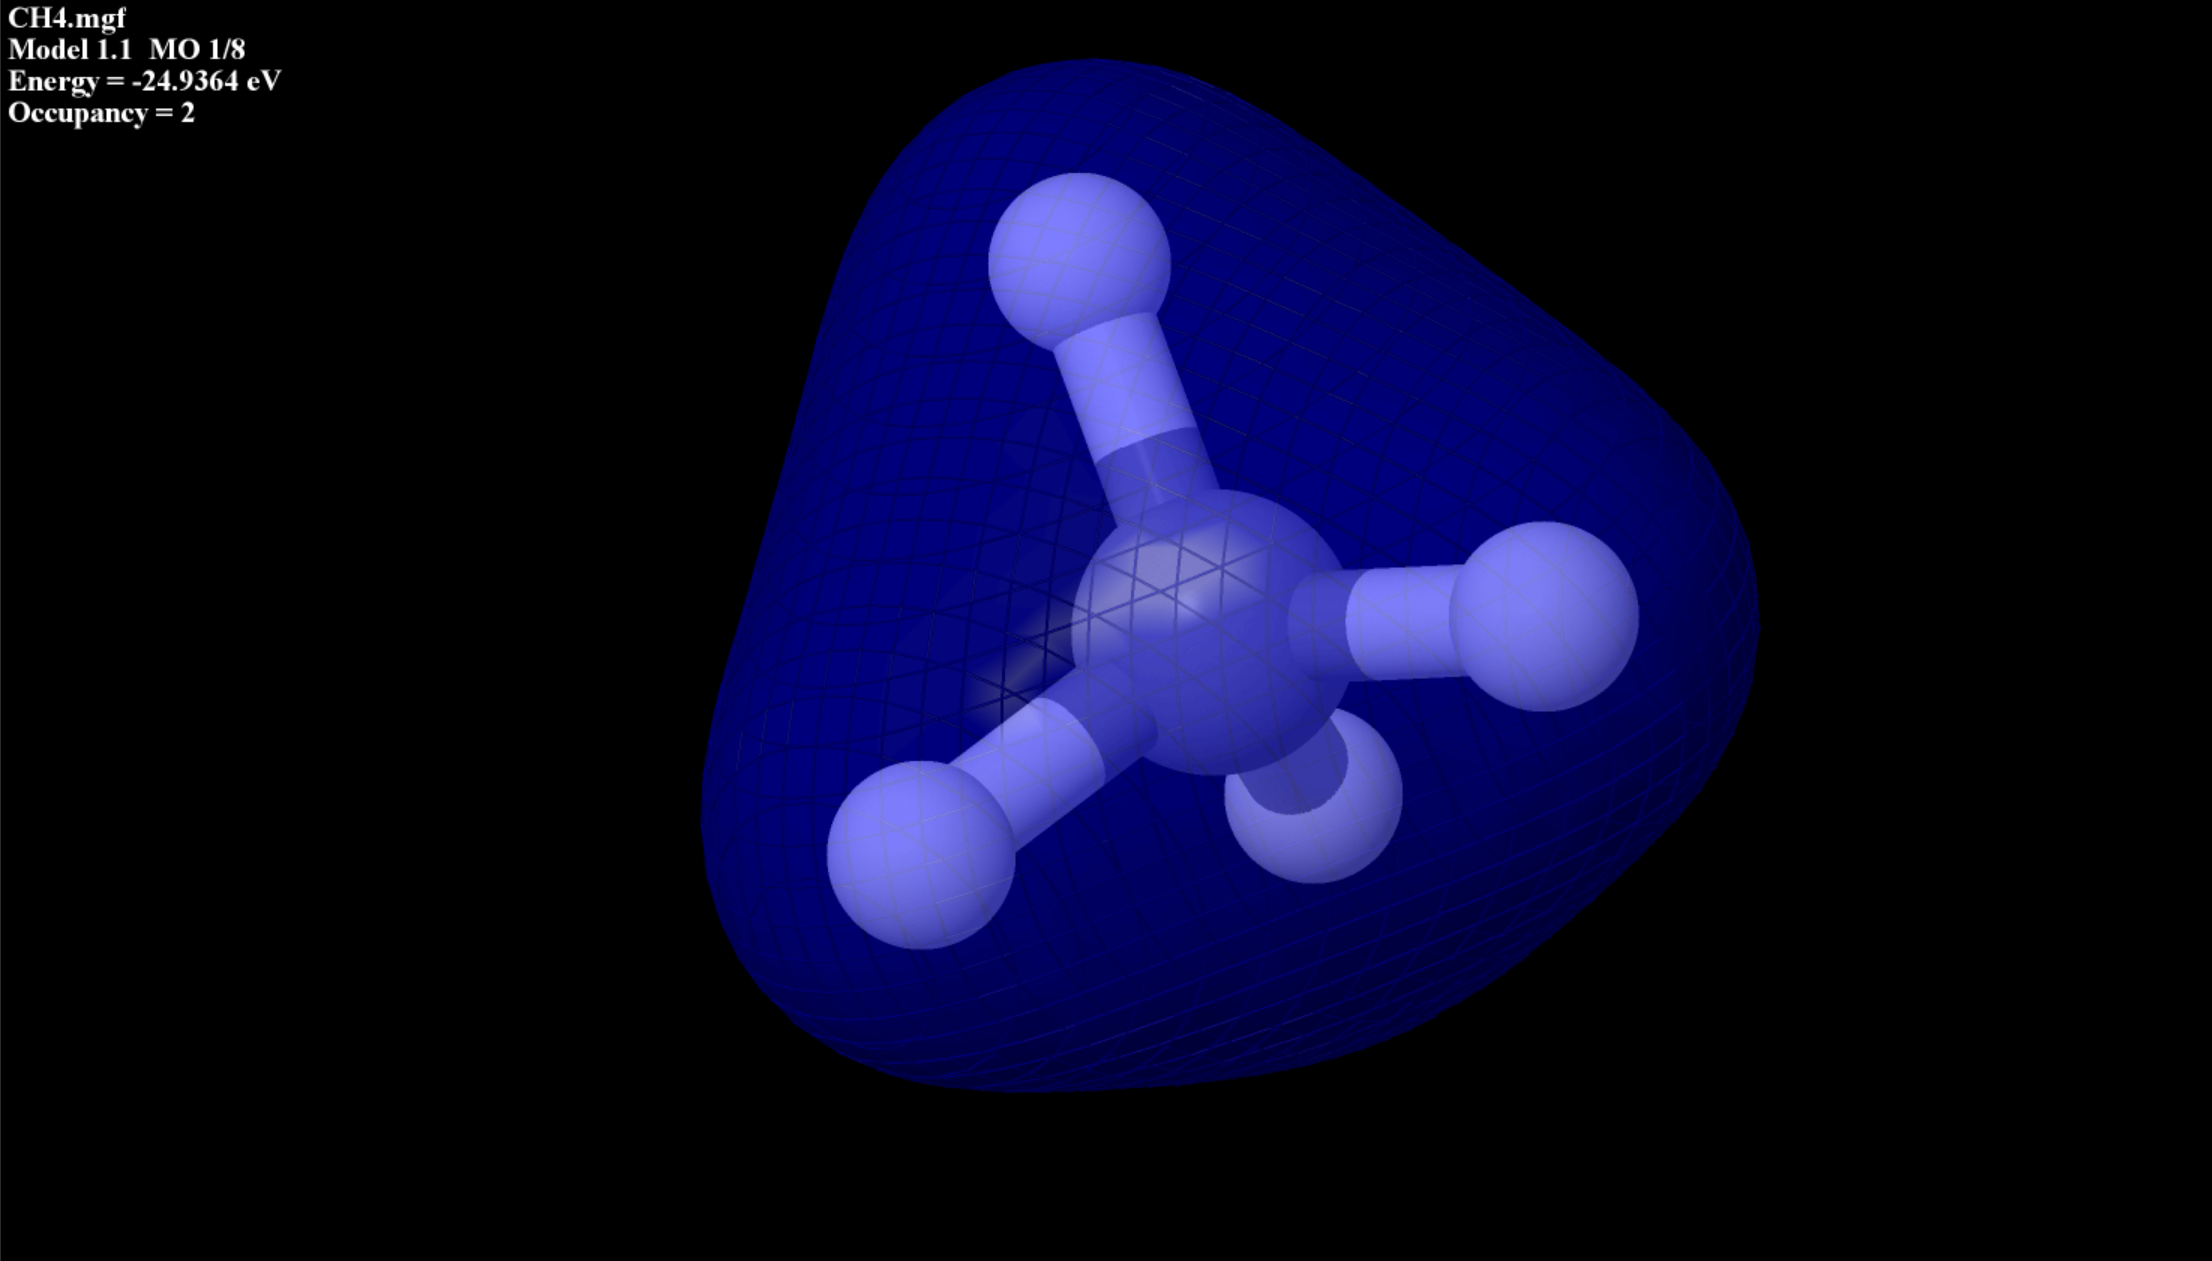
\includegraphics[width=\textwidth]{images-OM/MO 1 - CH4.png}
        \caption{OM 1}
        \label{fig:}
    \end{subfigure}
    \hspace{0.5cm}
    \begin{subfigure}{0.48\textwidth}
        \centering
        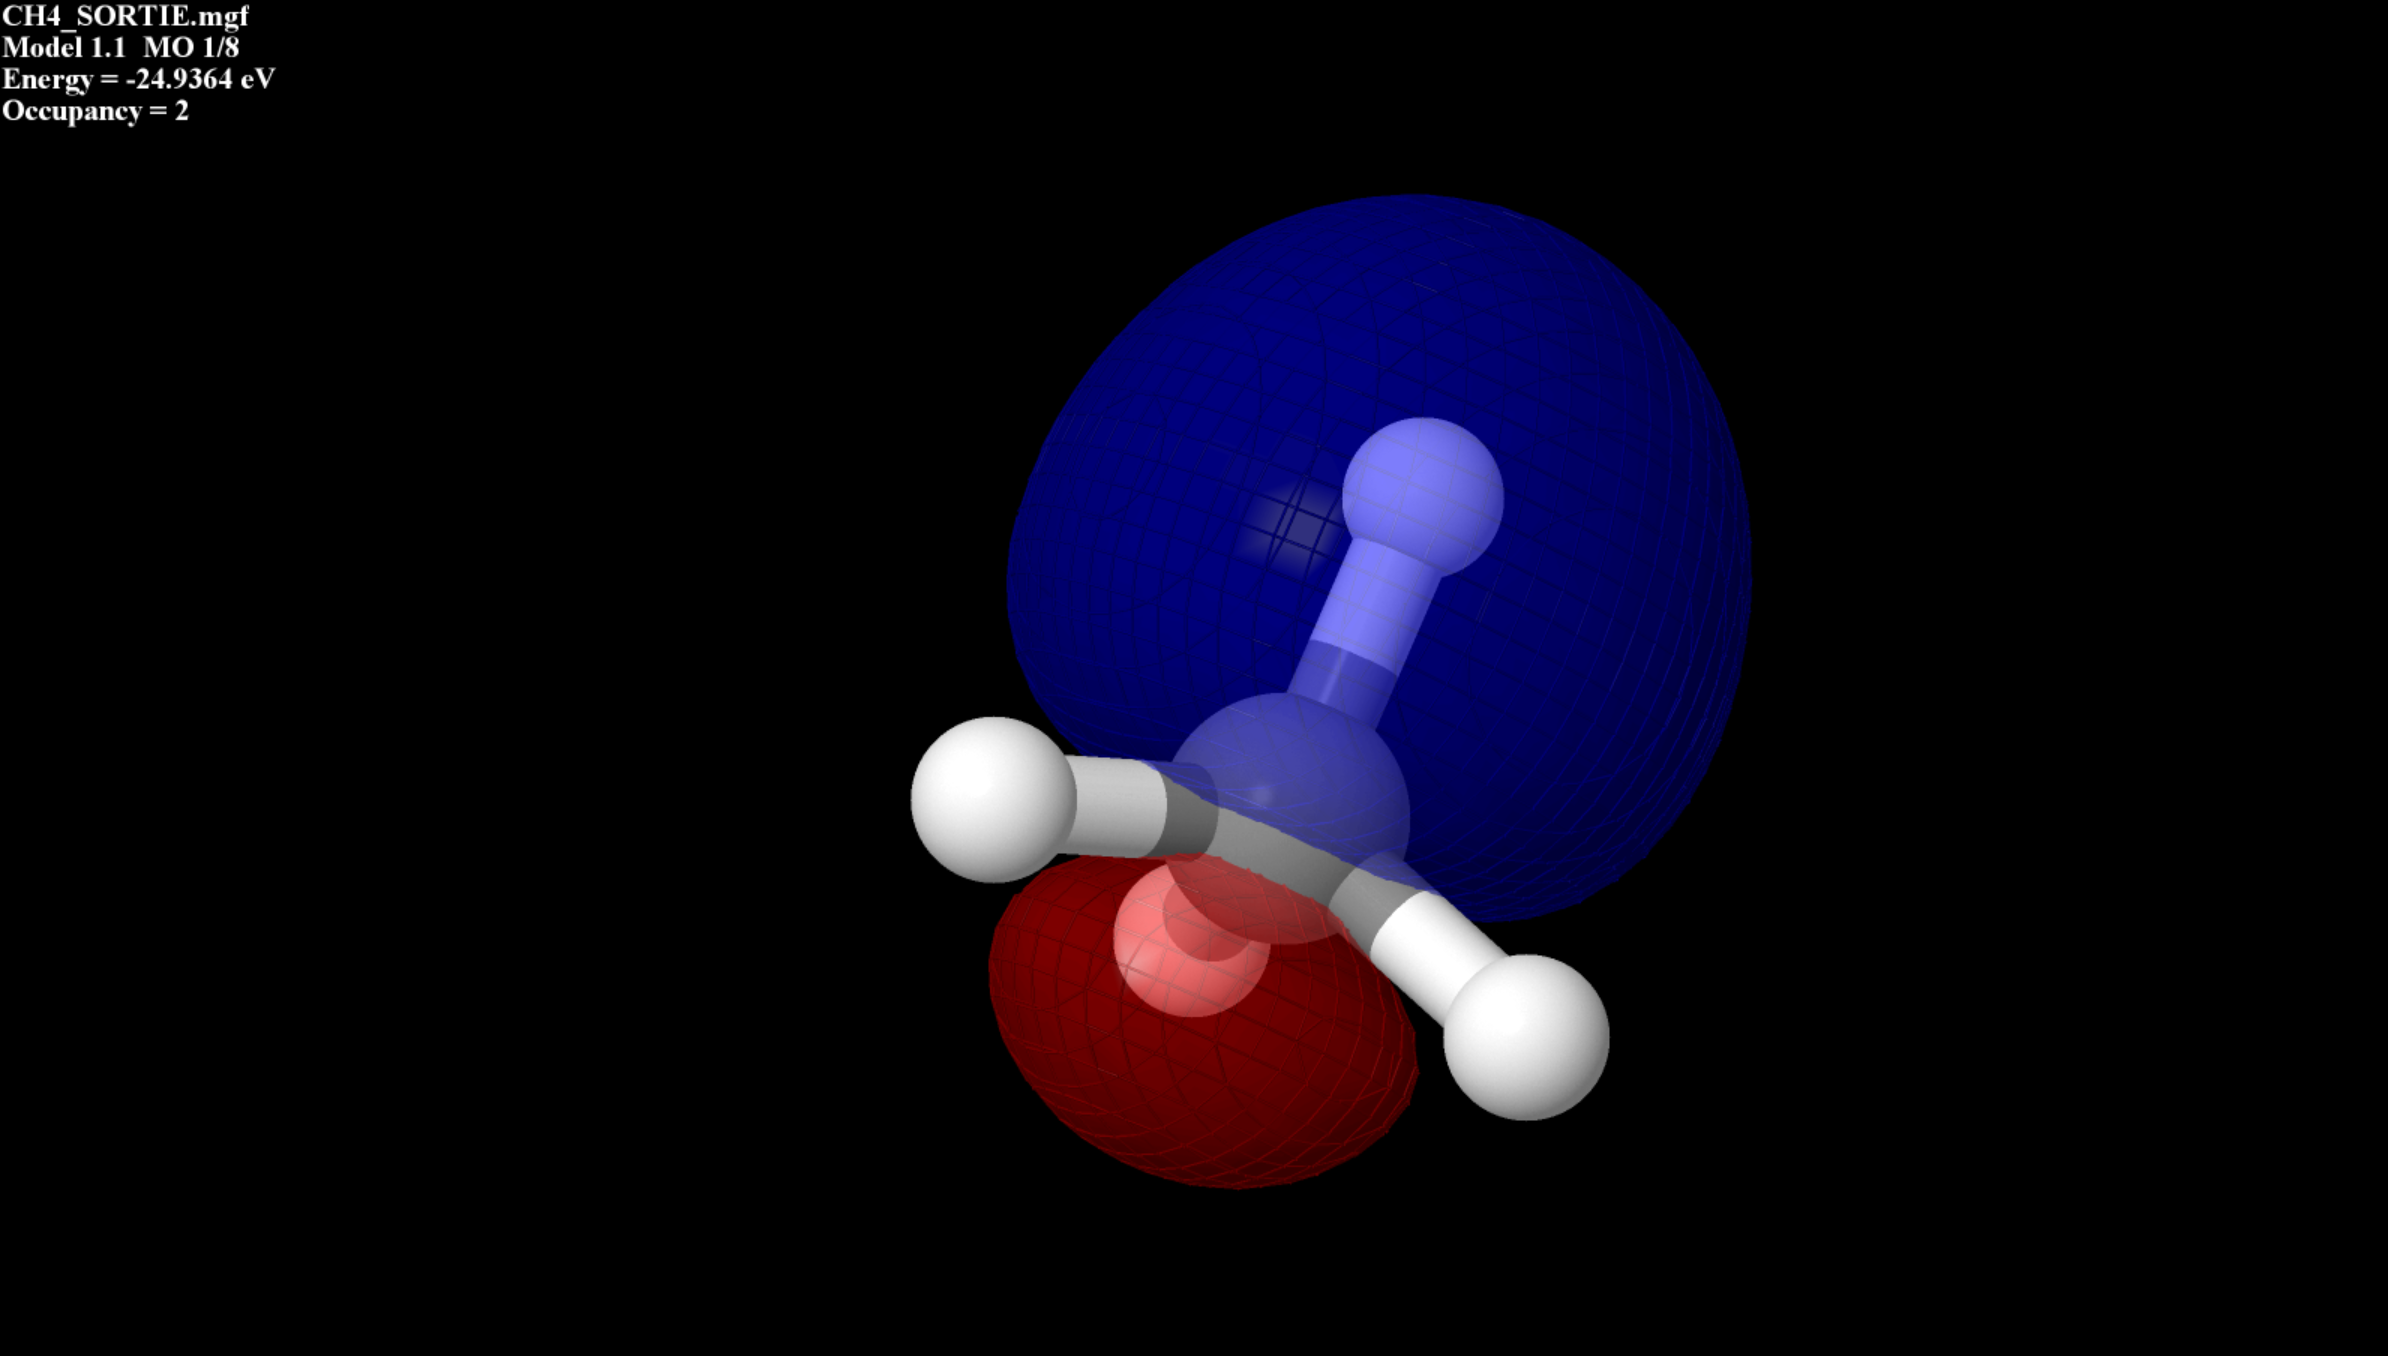
\includegraphics[width=\textwidth]{images-OM-Final/Sortie_MO 1 - CH4.png}
        \caption{OM\_output 1}
        \label{fig:}
    \end{subfigure}
    \caption{Visualisation \& Comparaison des OM n°1}
\end{figure}

Ici l'OM 1 ressemblait énormément à la 2s du carbone, et cela se confirmait via le fichier mgf avec un coefficient majoritaire sur la 2s$_C$ parmi les 4 OA du carbone (+ de 99\%). Cependant lorsque l'on visualise l'OM 1 en sortie de programme, celle-ci est localisée sur la liaison C-H$_1$, et l'on voit une belle hybridation sp$^3$. Cela prouve que l'on ne peut pas uniquement se fier aux représentations surfaciques des orbitales pour étudier la localisation des électrons. Puisque malgré que la représentation de l'OM 1 soit véridique, les électrons se trouvent uniquement dans les volumes délimités par l'OM 1 sortante (notre programme restreint la délimitation).

\begin{figure}[H]
    \centering
    \begin{subfigure}{0.48\textwidth}
        \centering
        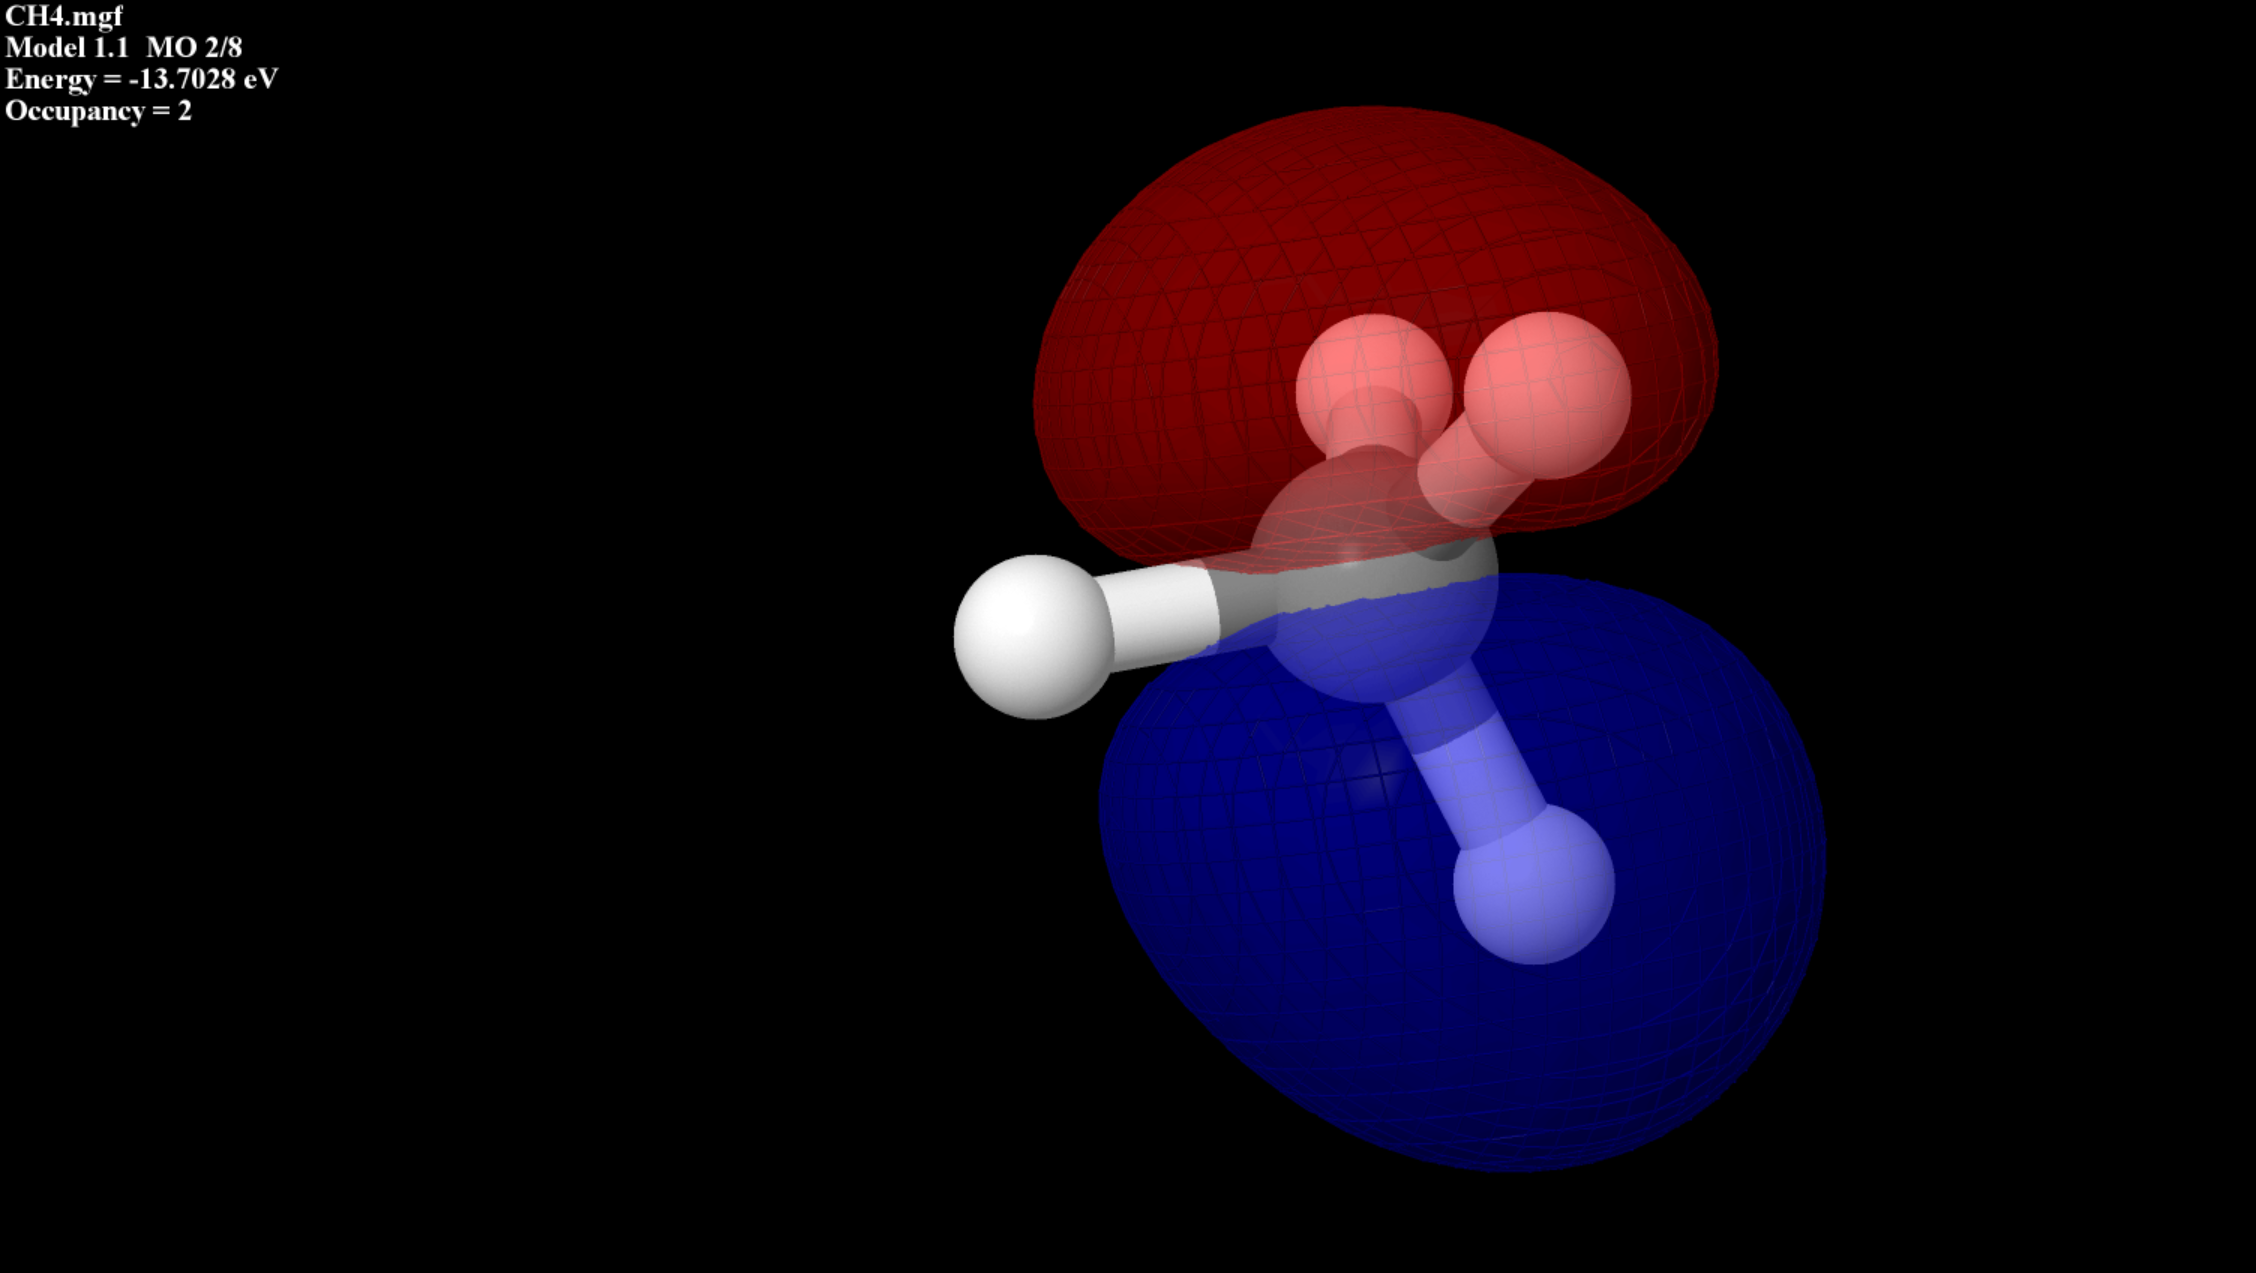
\includegraphics[width=\textwidth]{images-OM/MO 2 - CH4.png}
        \caption{OM 2}
        \label{fig:}
    \end{subfigure}
    \hspace{0.5cm}
    \begin{subfigure}{0.48\textwidth}
        \centering
        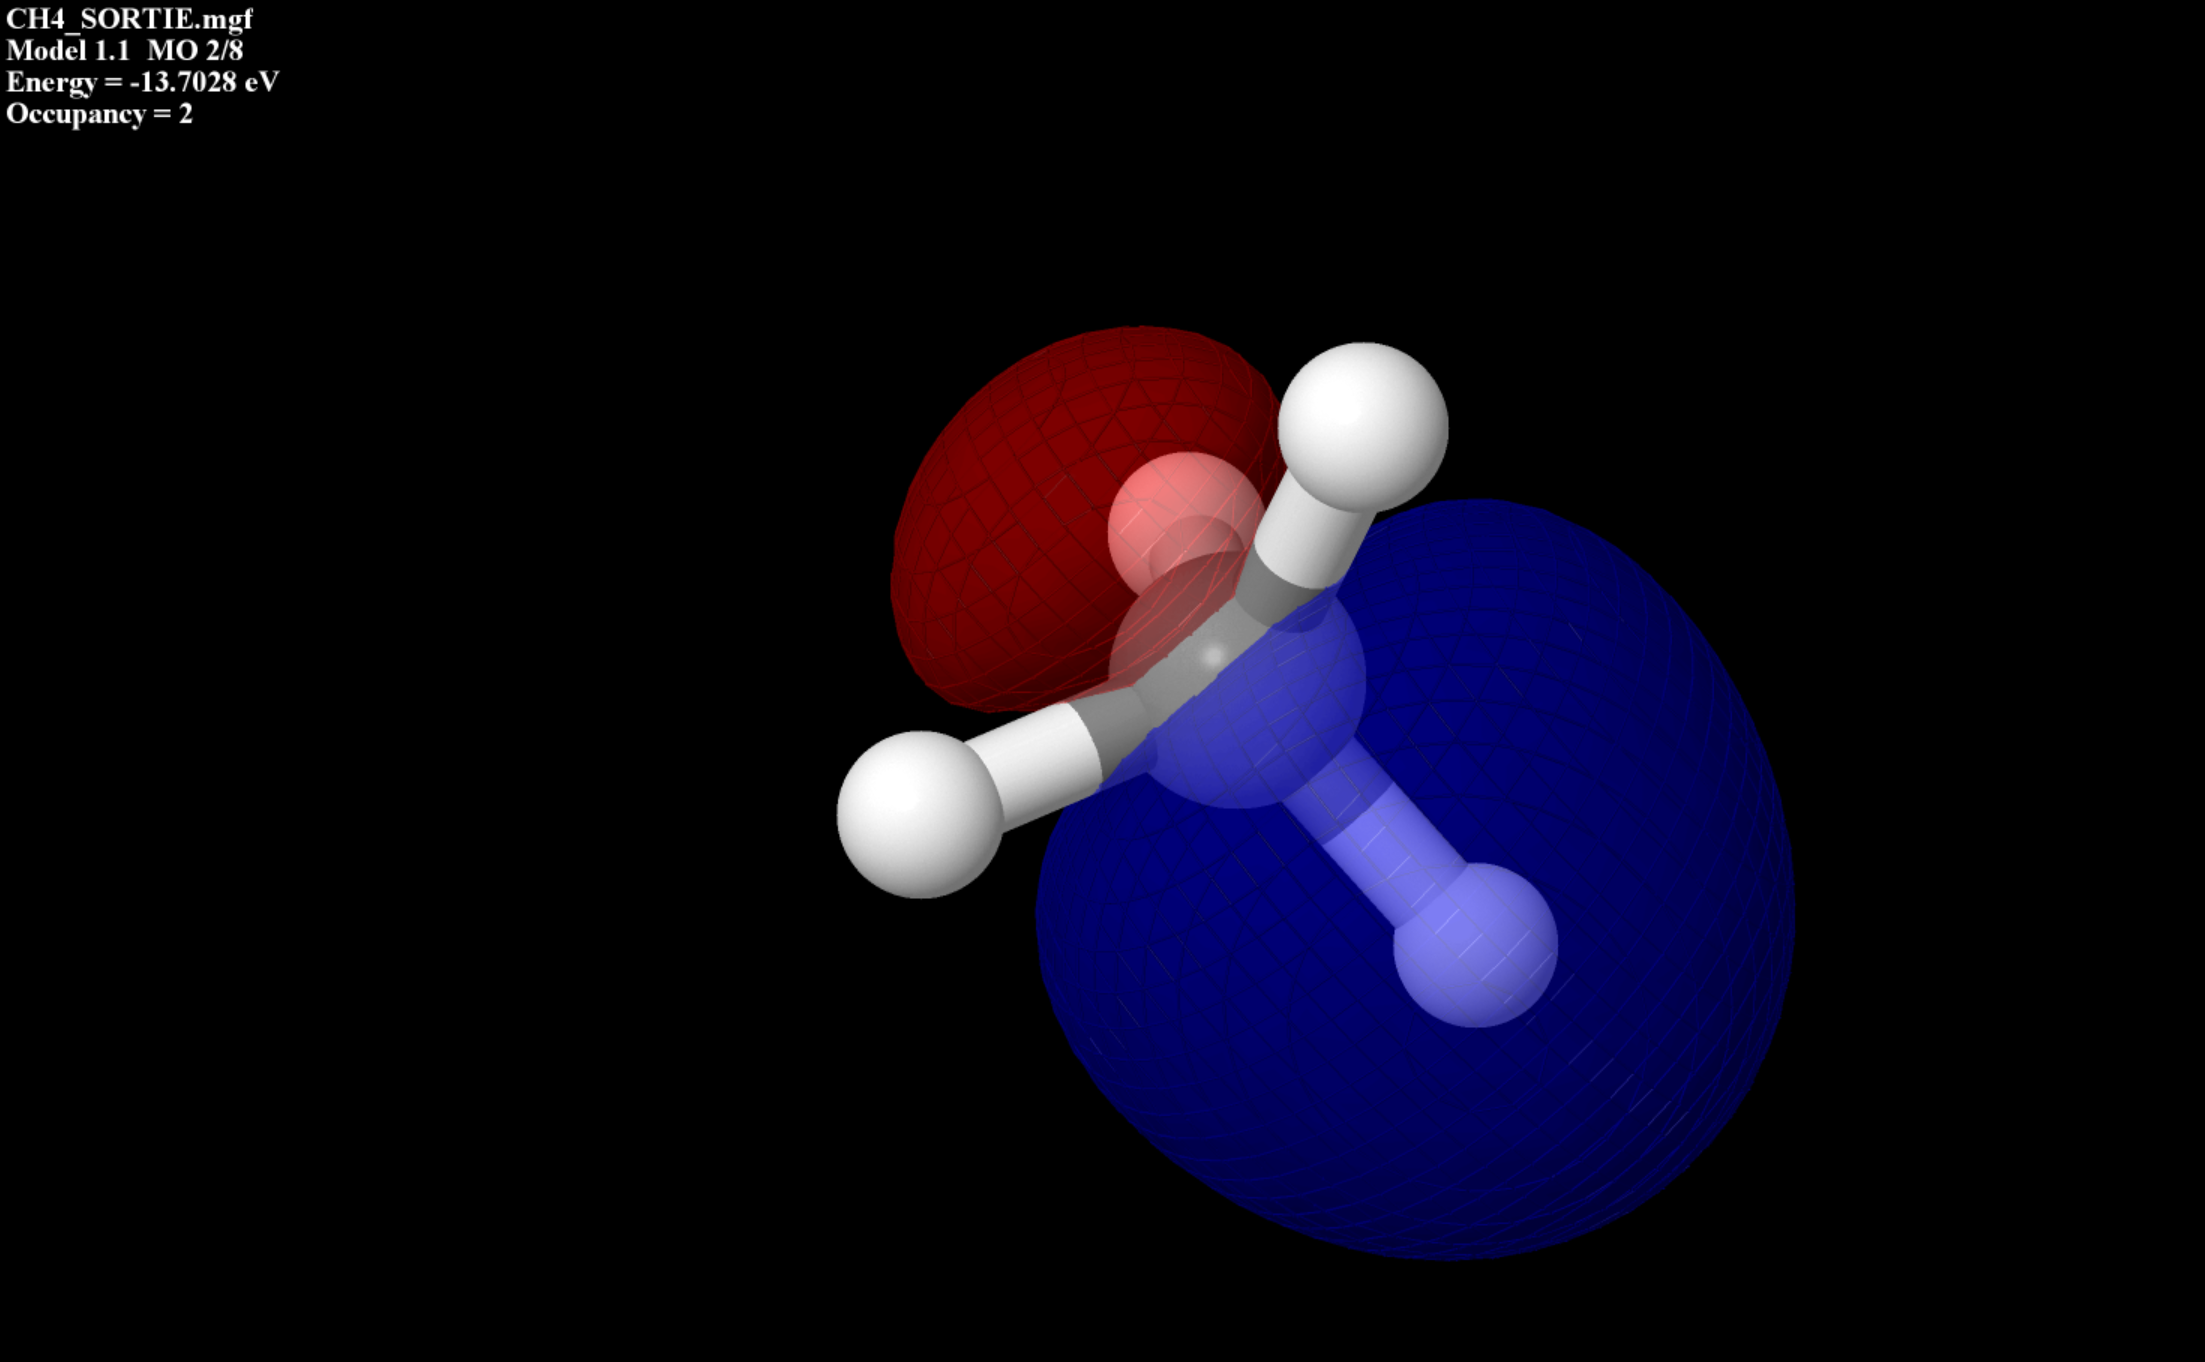
\includegraphics[width=\textwidth]{images-OM-Final/Sortie_MO 2bis - CH4.png}
        \caption{OM\_output 2}
        \label{fig:}
    \end{subfigure}
    \caption{Visualisation \& Comparaison des OM n°2}
\end{figure}

\begin{figure}[H]
    \centering
    \begin{subfigure}{0.48\textwidth}
        \centering
        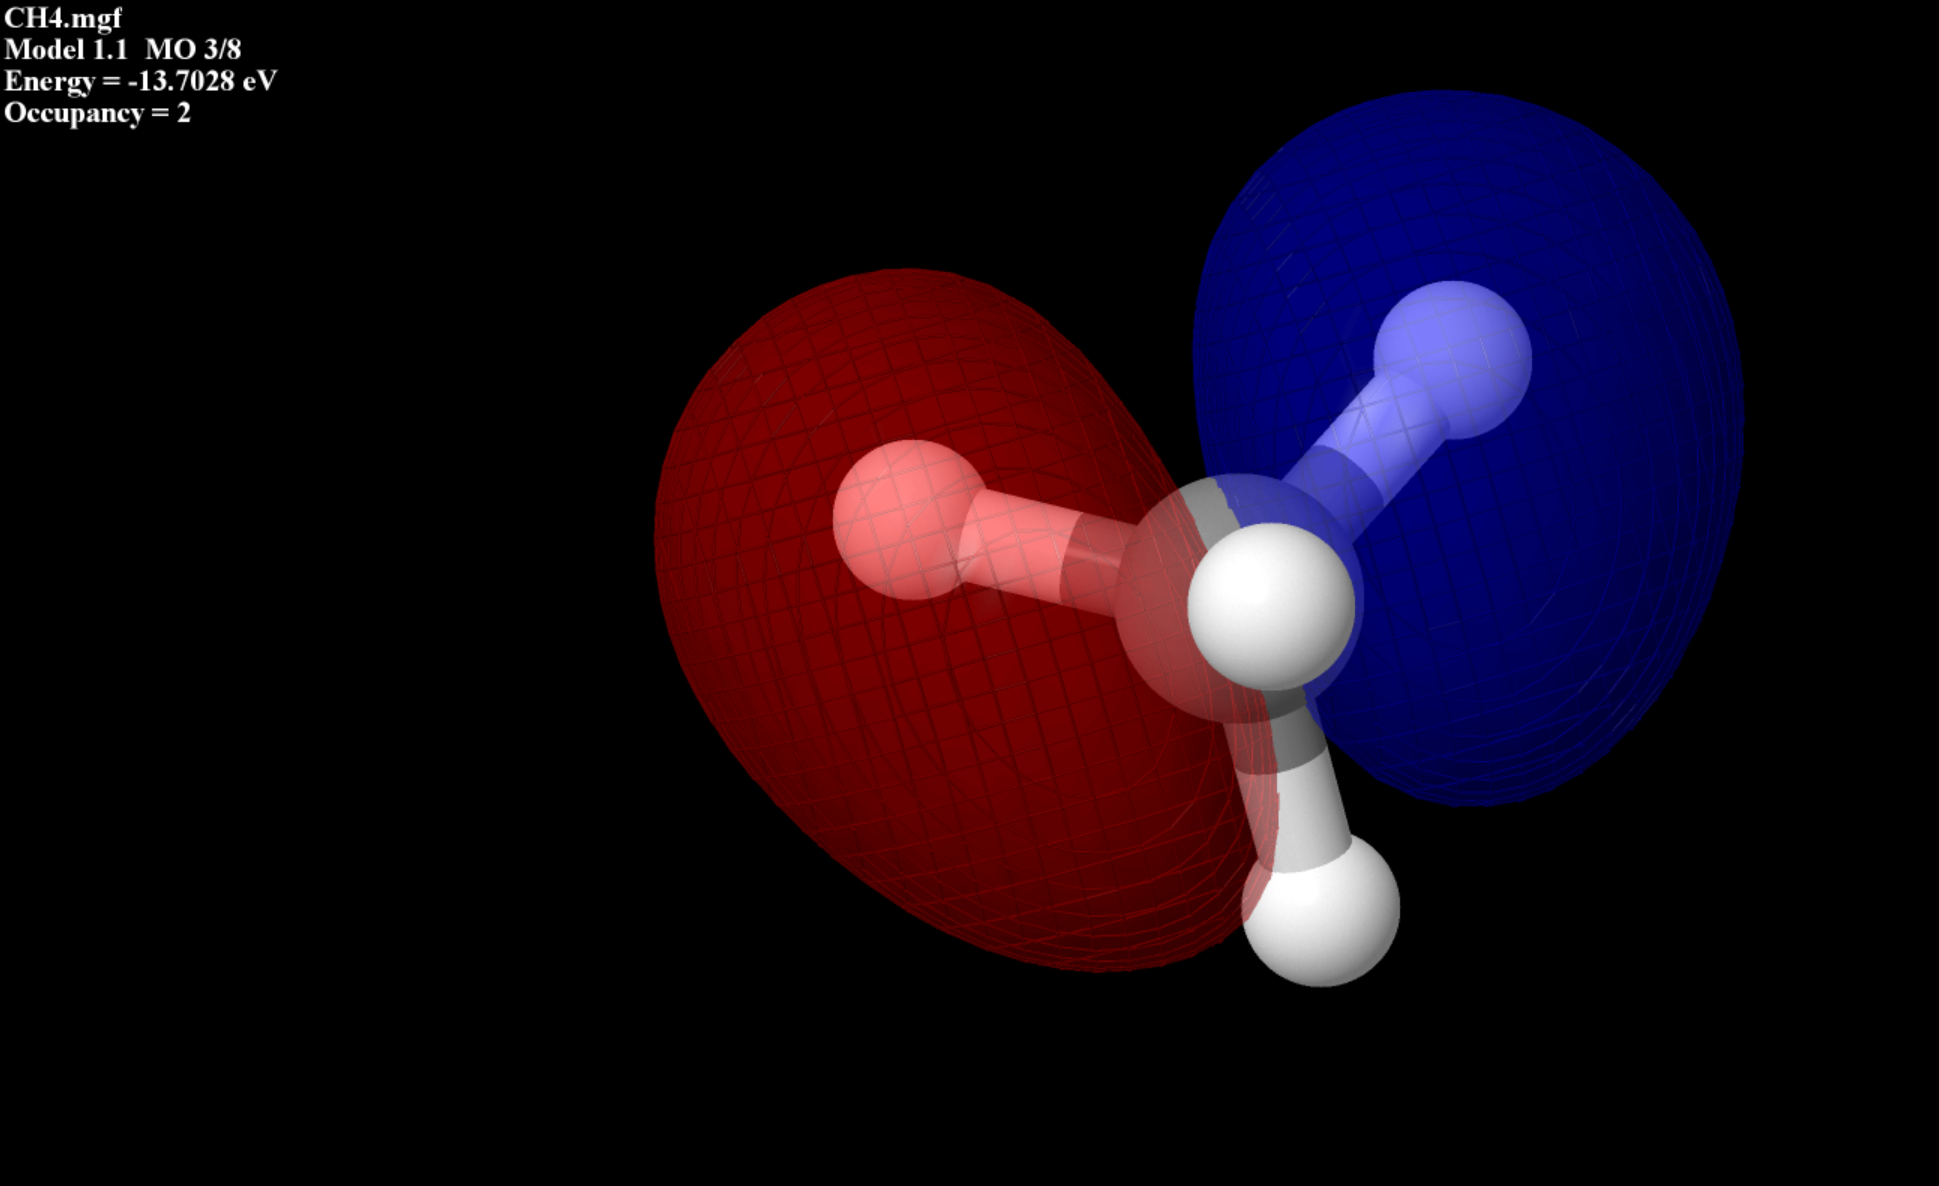
\includegraphics[width=\textwidth]{images-OM/MO 3 - CH4.png}
        \caption{OM 3}
        \label{fig:}
    \end{subfigure}
    \hspace{0.5cm}
    \begin{subfigure}{0.48\textwidth}
        \centering
        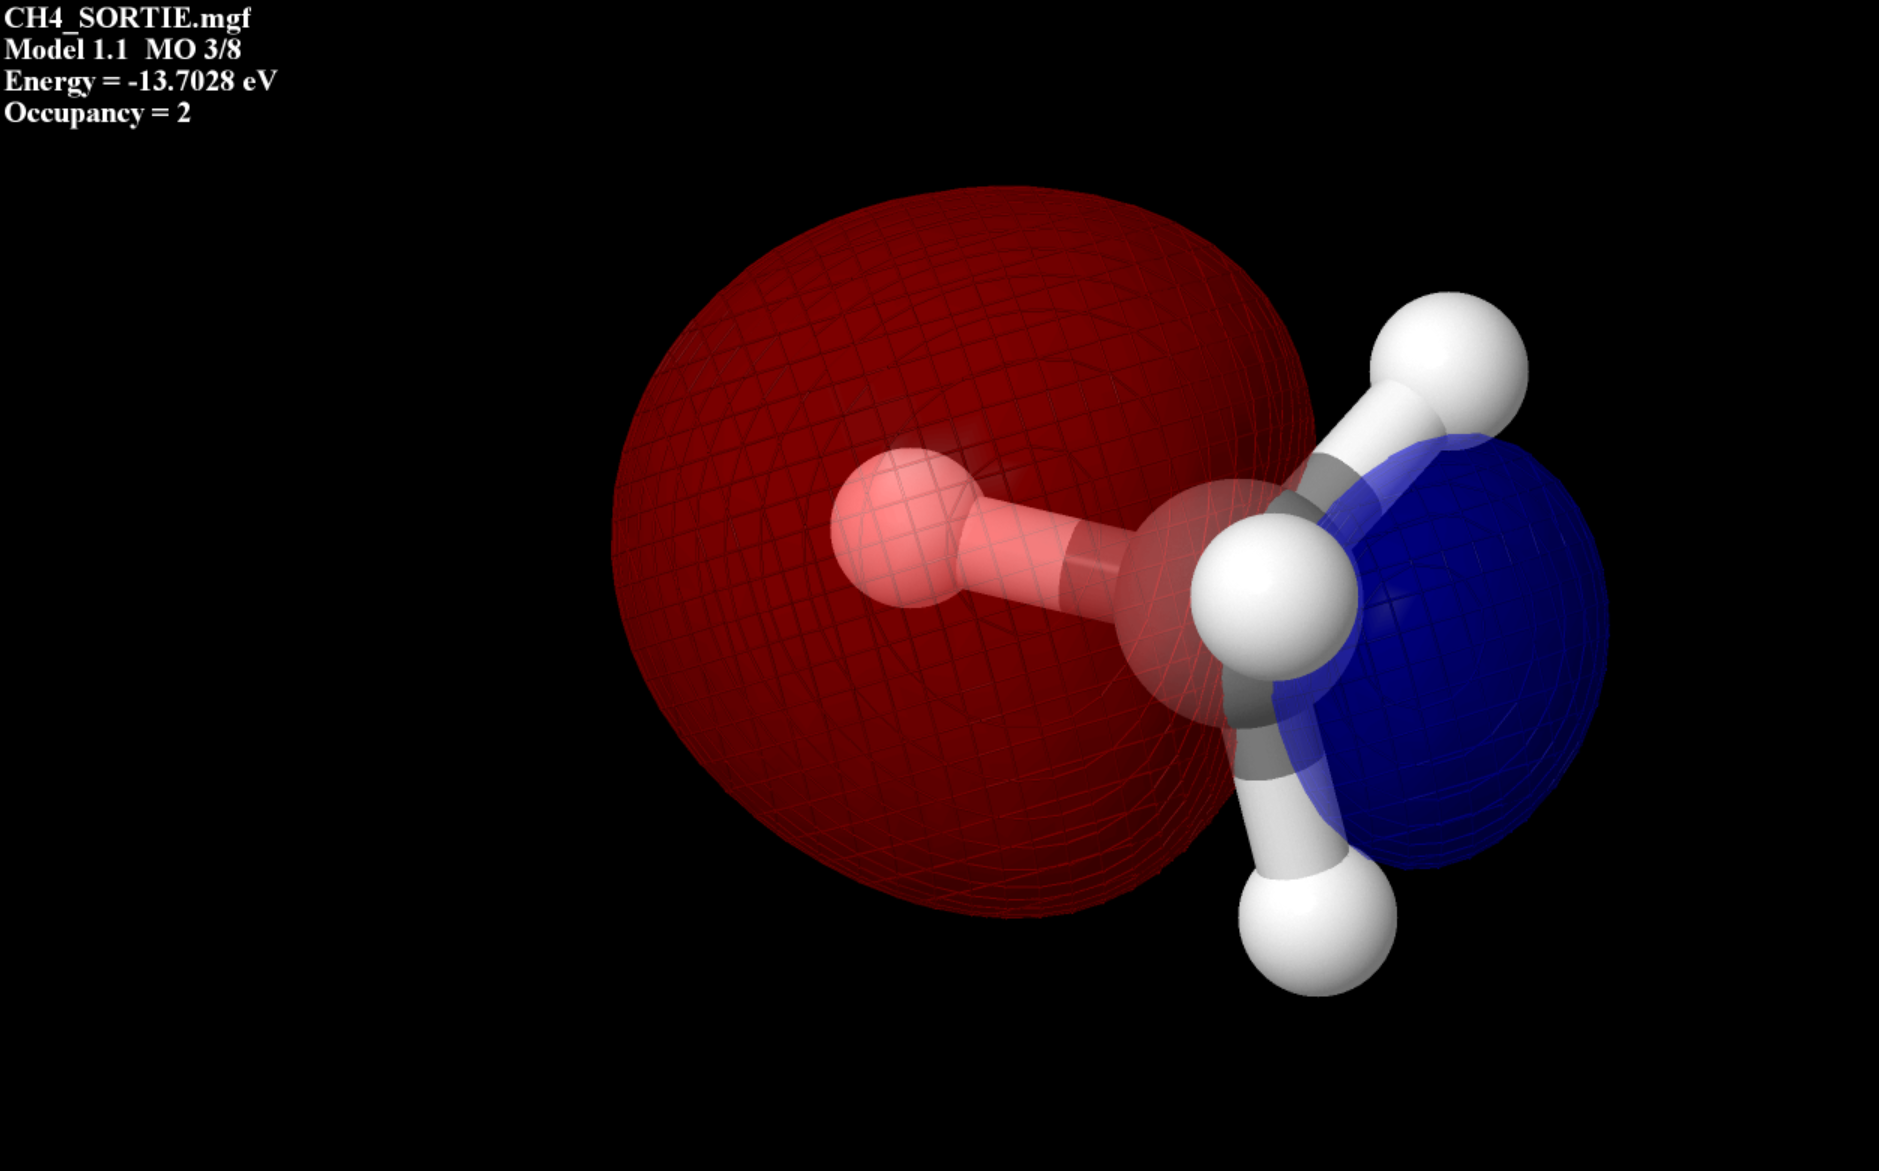
\includegraphics[width=\textwidth]{images-OM-Final/Sortie_MO 3bis - CH4.png}
        \caption{OM\_output 3}
        \label{fig:}
    \end{subfigure}
    \caption{Visualisation \& Comparaison des OM n°3}
\end{figure}

A première vue, on peut considérer que la visualisation de l'OM 3 localisée n'est pas cohérente avec son OM initiale et avec les trois autres OM localisées. Cependant, on ne s'intéresse pas au signe des lobes et en ce qui concerne la couverture de l'orbitale rouge, celle-ci est parfaitement localisée sur la liaison C-H. On observe donc une OM résultant du recouvrement d’orbitales de type sp$^3$.
%A première vue, on peut considérer que la visualisation de l'OM 3 localisée n'est pas cohérente avec son OM initiale. Cependant, le lobe rouge englobe légèrement plus le carbone même s'il englobe tout autant son atome d'hydrogène. Cela pourrait expliquer que le signe rouge soit le lobe prédominant de la liaison (de type sp$^3$).

\begin{figure}[H]
    \centering
    \begin{subfigure}{0.48\textwidth}
        \centering
        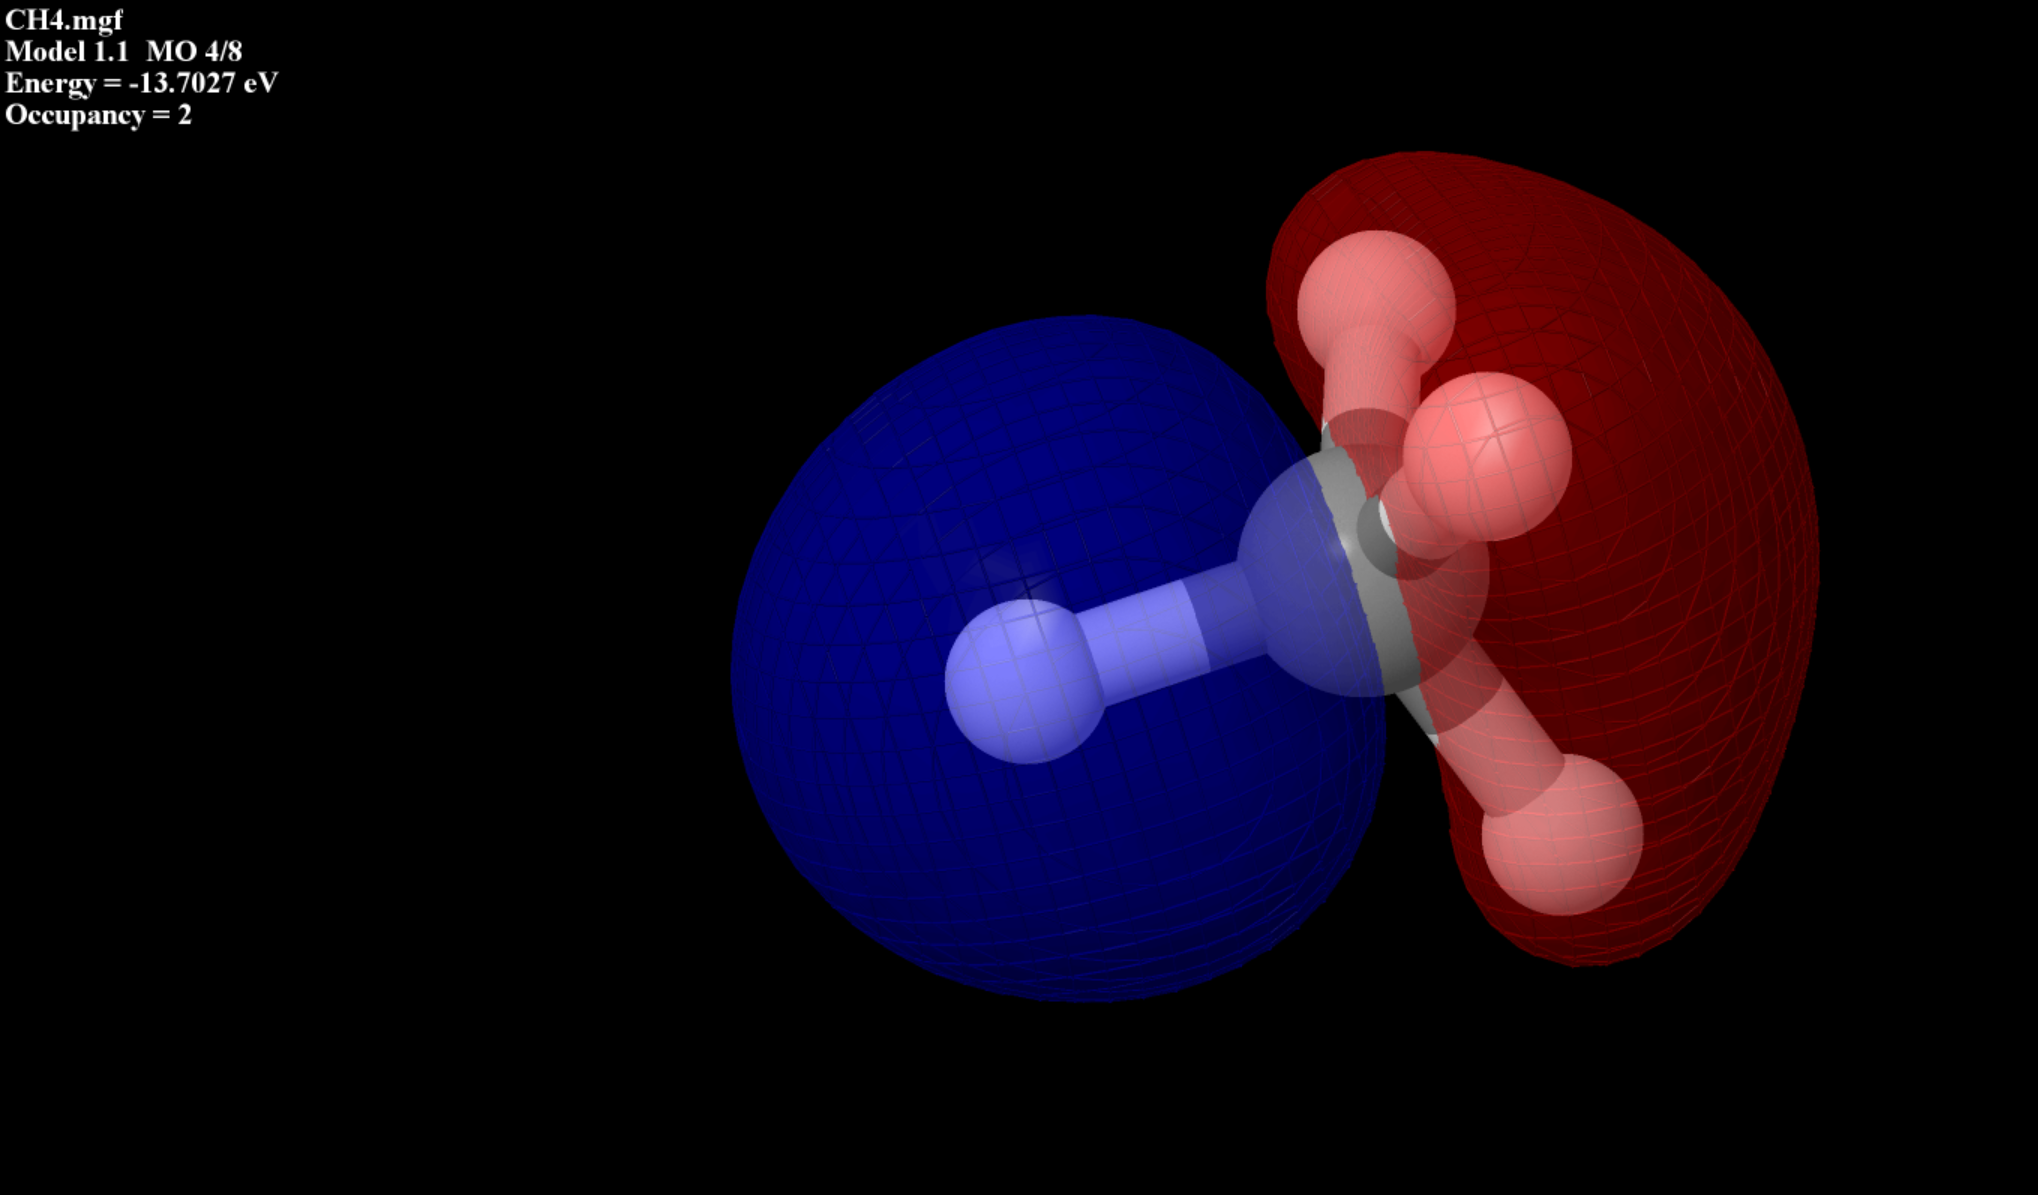
\includegraphics[width=\textwidth]{images-OM/MO 4 - CH4.png}
        \caption{OM 4}
        \label{fig:}
    \end{subfigure}
    \hspace{0.5cm}
    \begin{subfigure}{0.48\textwidth}
        \centering
        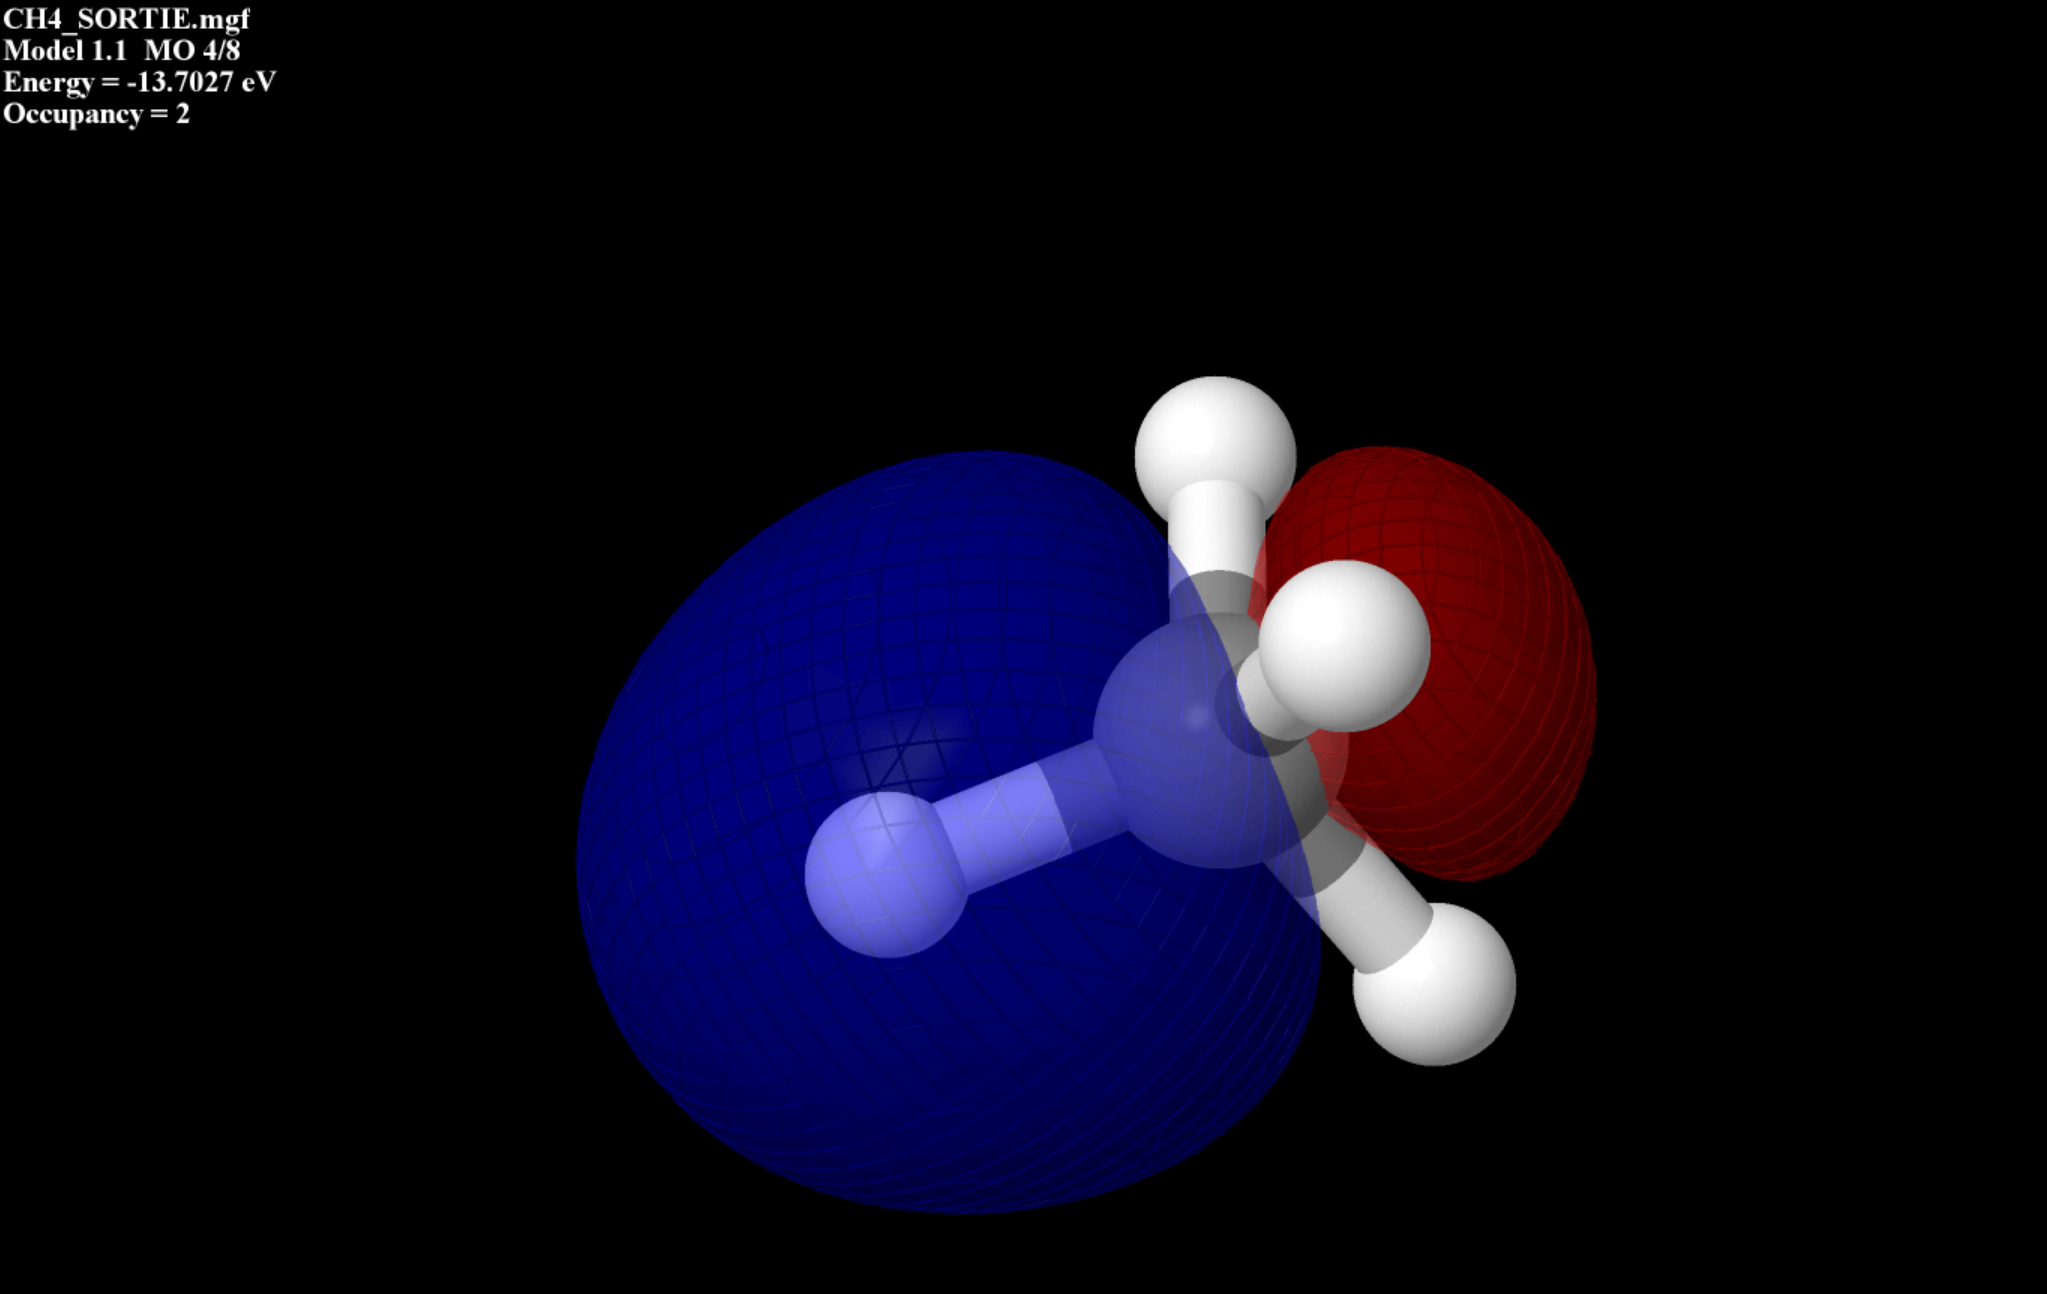
\includegraphics[width=\textwidth]{images-OM-Final/Sortie_MO 4bis - CH4.png}
        \caption{OM\_output 4}
        \label{fig:}
    \end{subfigure}
    \caption{Visualisation \& Comparaison des OM n°4}
\end{figure}

Pour les OM 2 et 4, la visualisation de celles-ci en sortie est \textbf{cohérente} avec leur OM non localisée puisque les lobes bleus englobant déjà la liaison C-H finissent par la recouvrir en exclusivité. Tandis que les lobes rouges suivent la forme de l'orbitale de type sp$^3$. 

\begin{figure}[H]
    \centering
    \begin{subfigure}{0.46\textwidth}
        \centering
        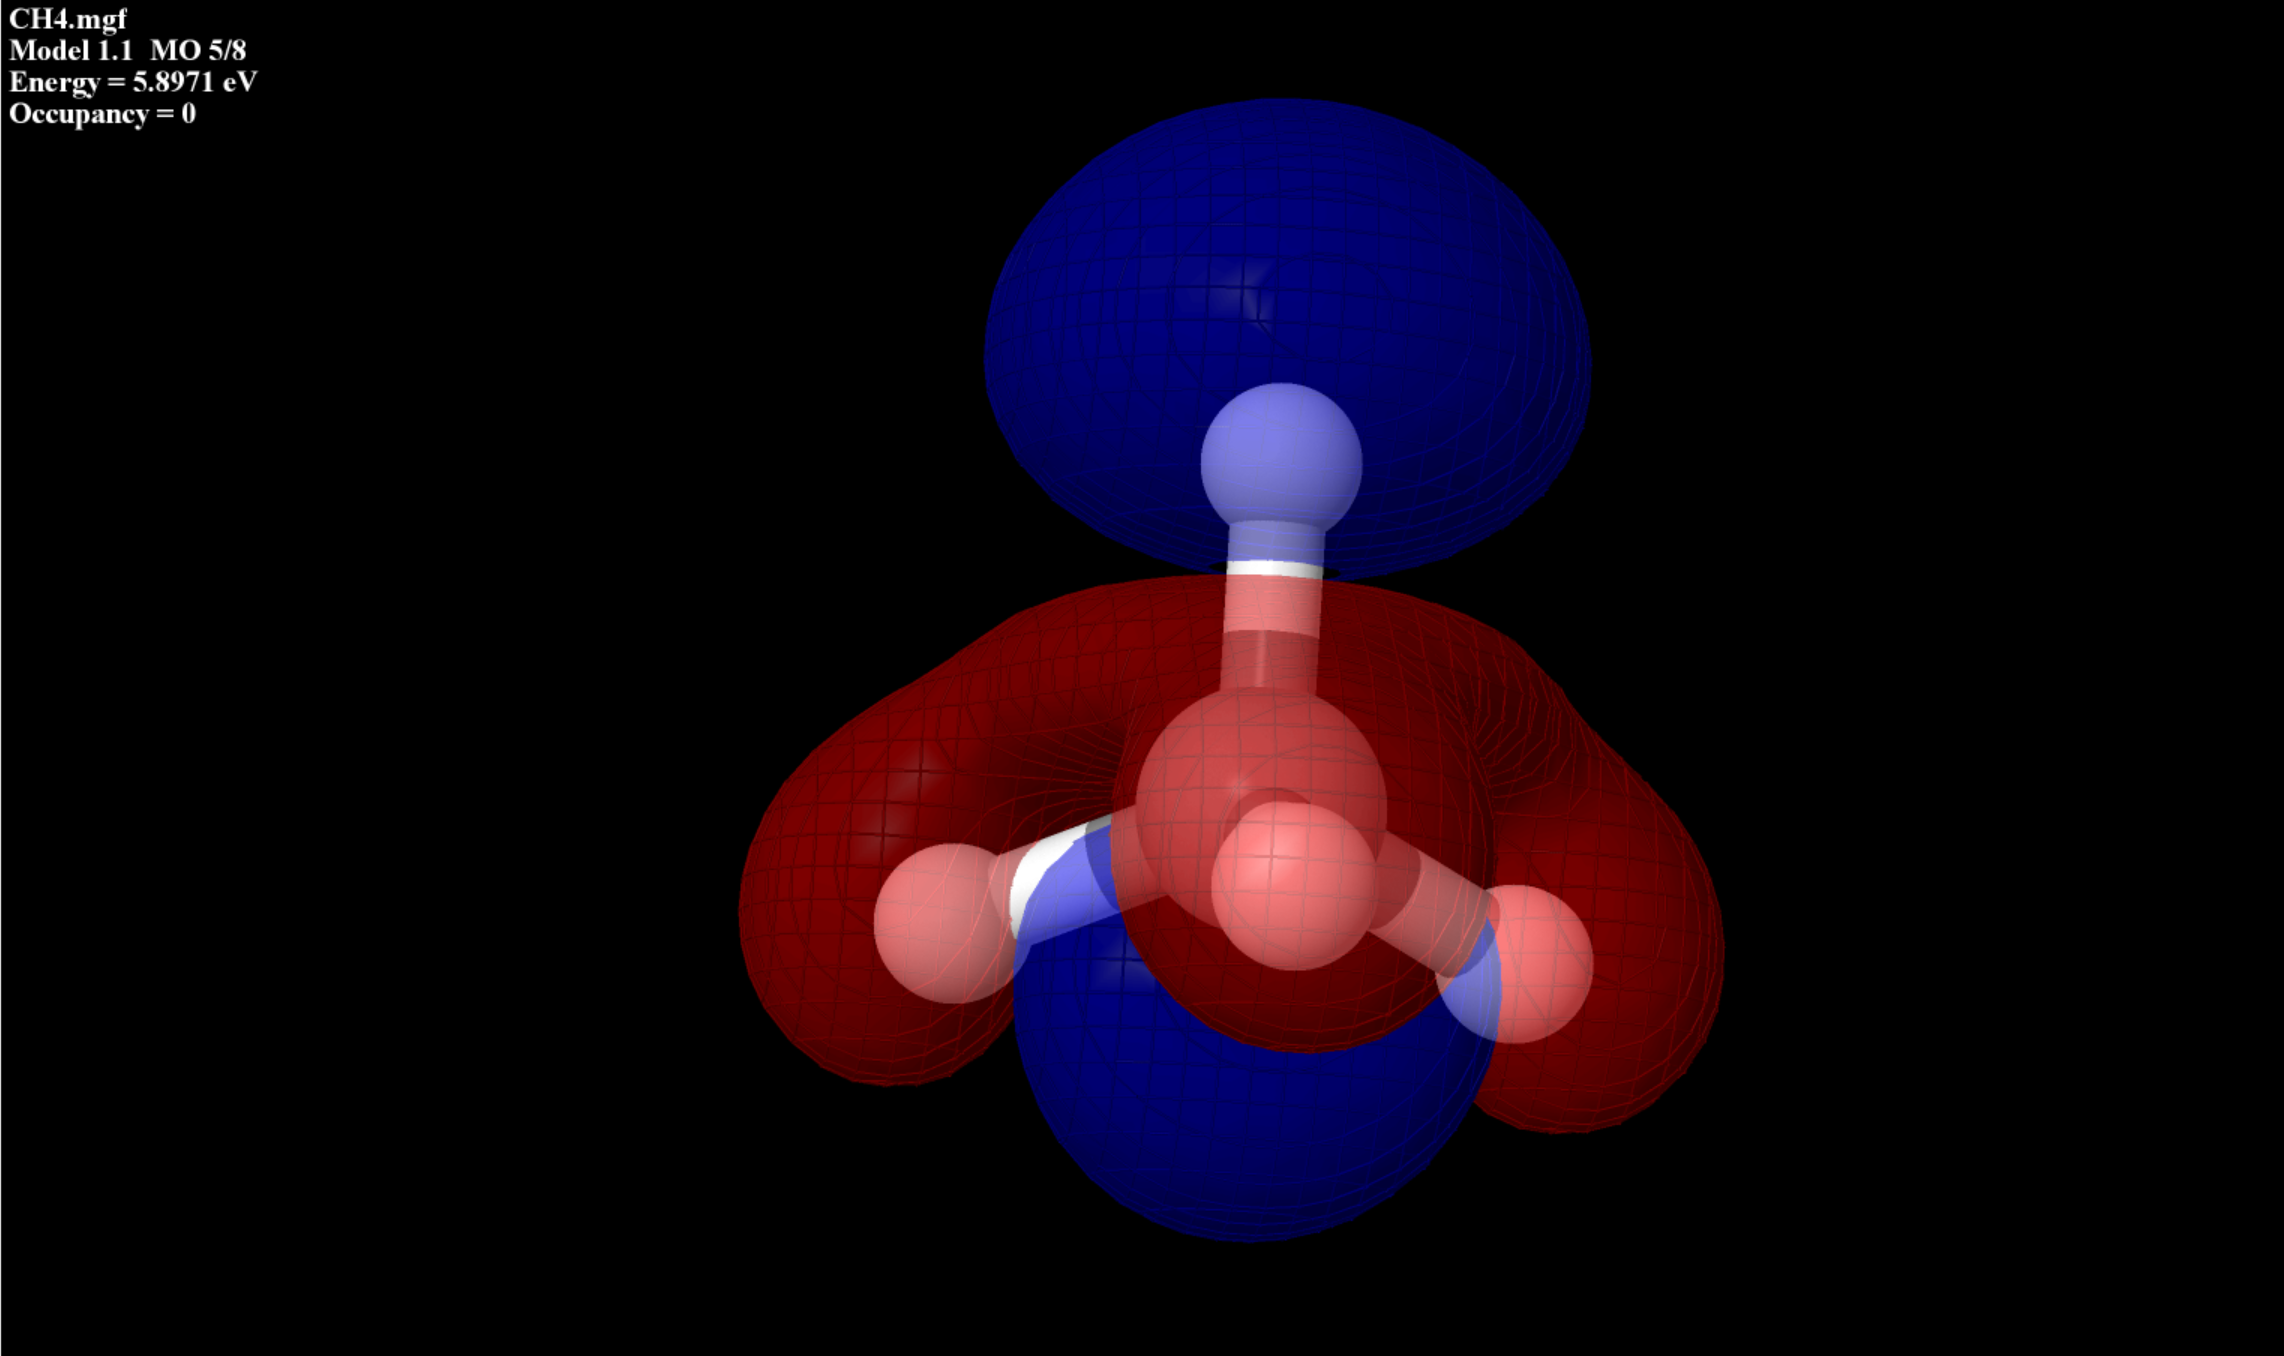
\includegraphics[width=\textwidth]{images-OM/MO 5 - CH4.png}
        \caption{OM 5}
        \label{fig:}
    \end{subfigure}
    \hspace{0.5cm}
    \begin{subfigure}{0.46\textwidth}
        \centering
        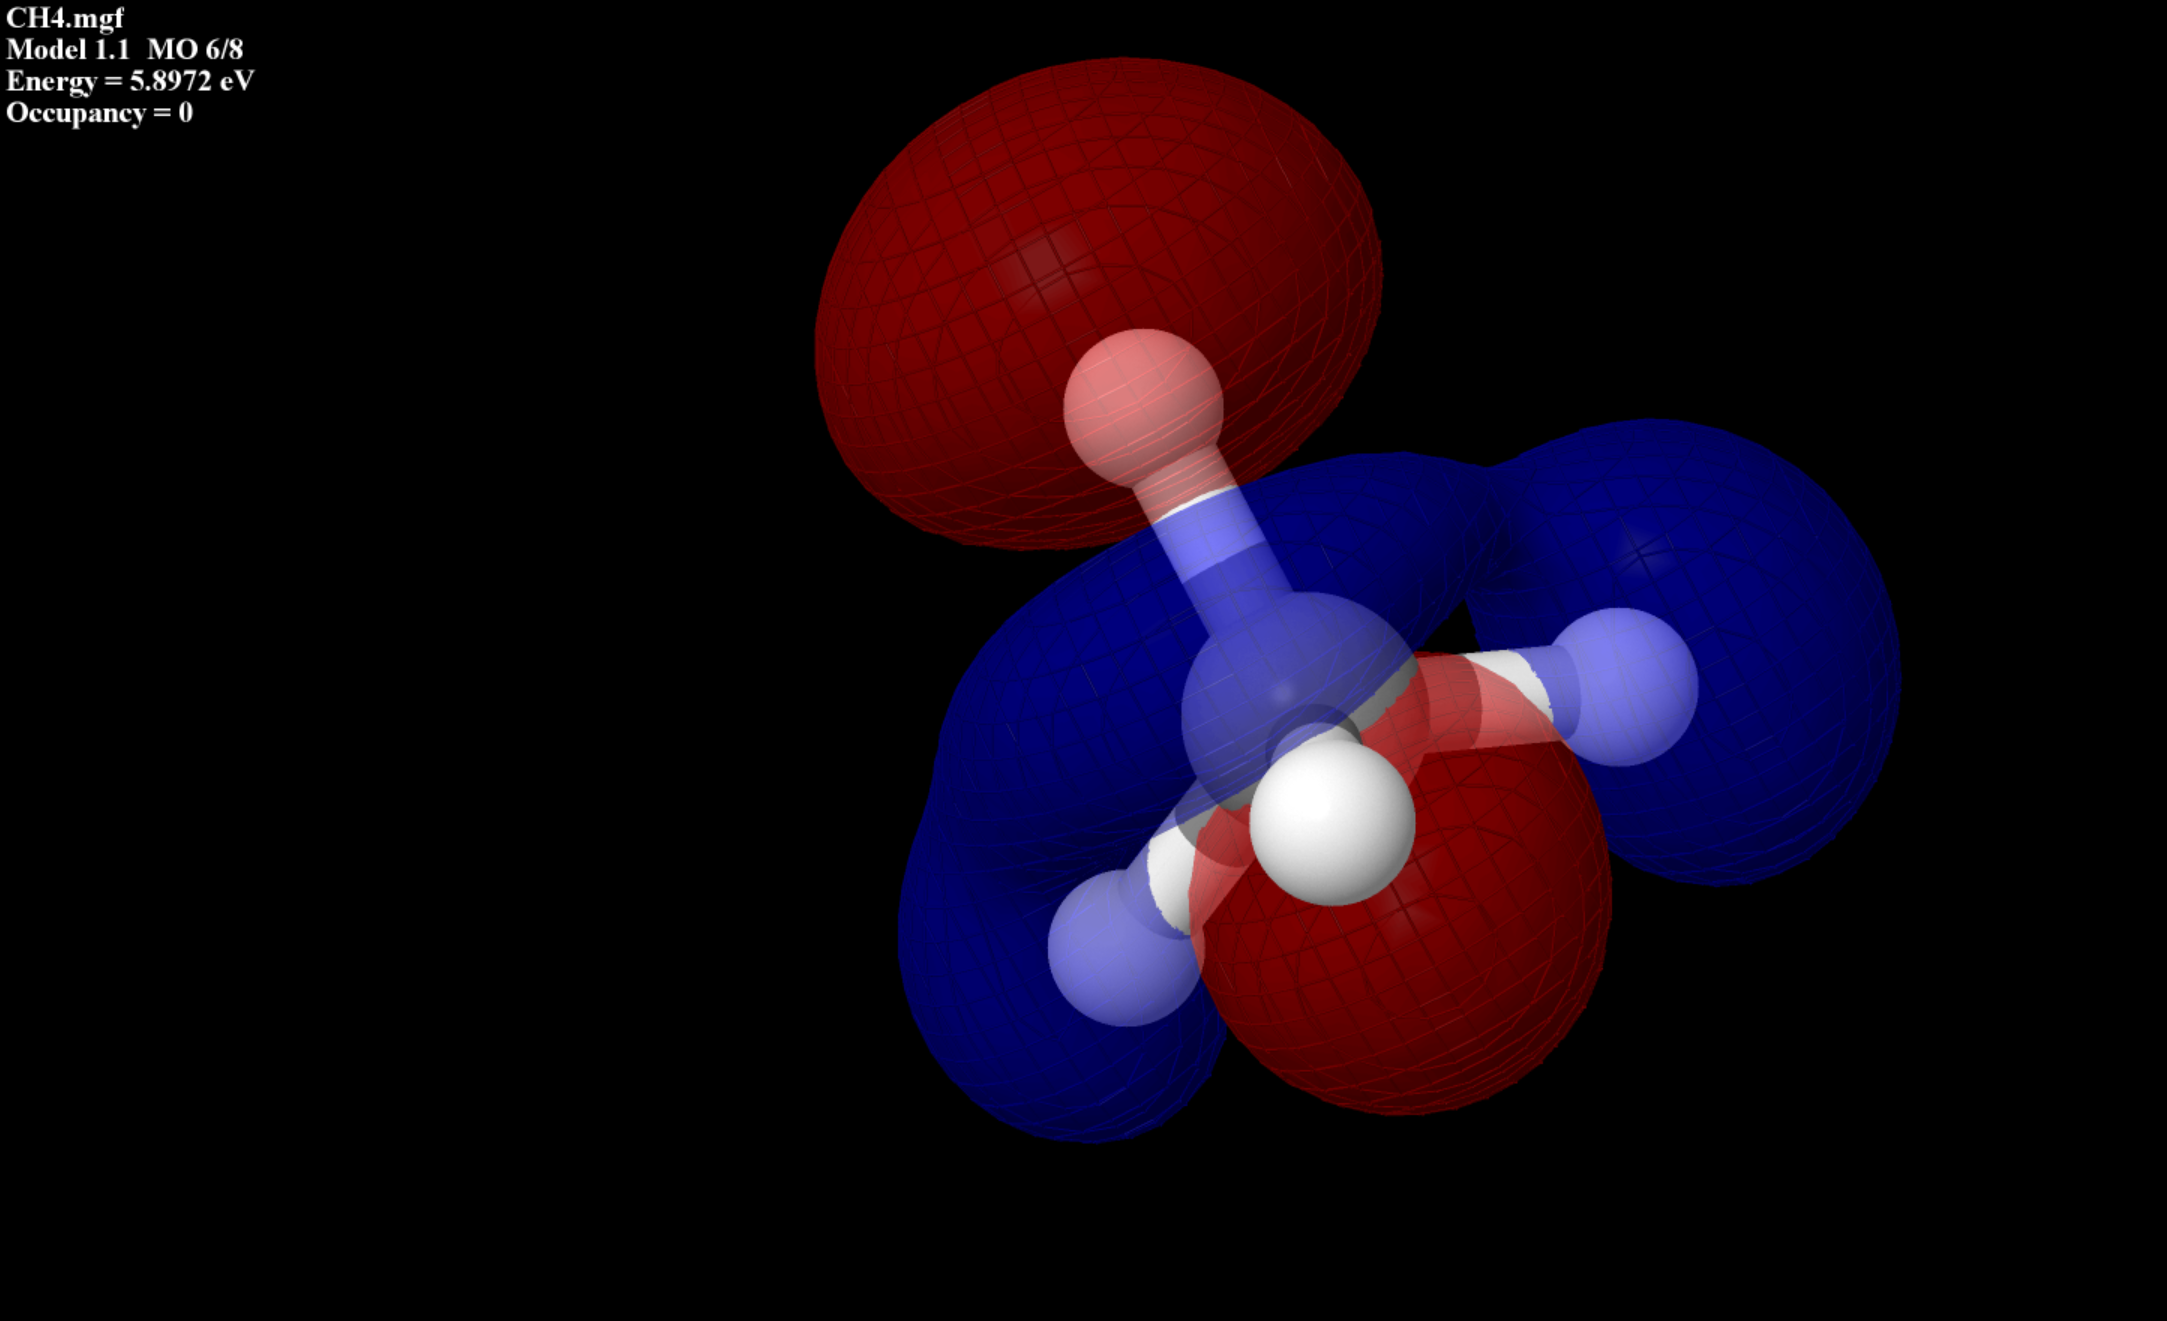
\includegraphics[width=\textwidth]{images-OM/MO 6 - CH4.png}
        \caption{OM 6}
        \label{fig:}
    \end{subfigure}
    \begin{subfigure}{0.48\textwidth}
        \centering
        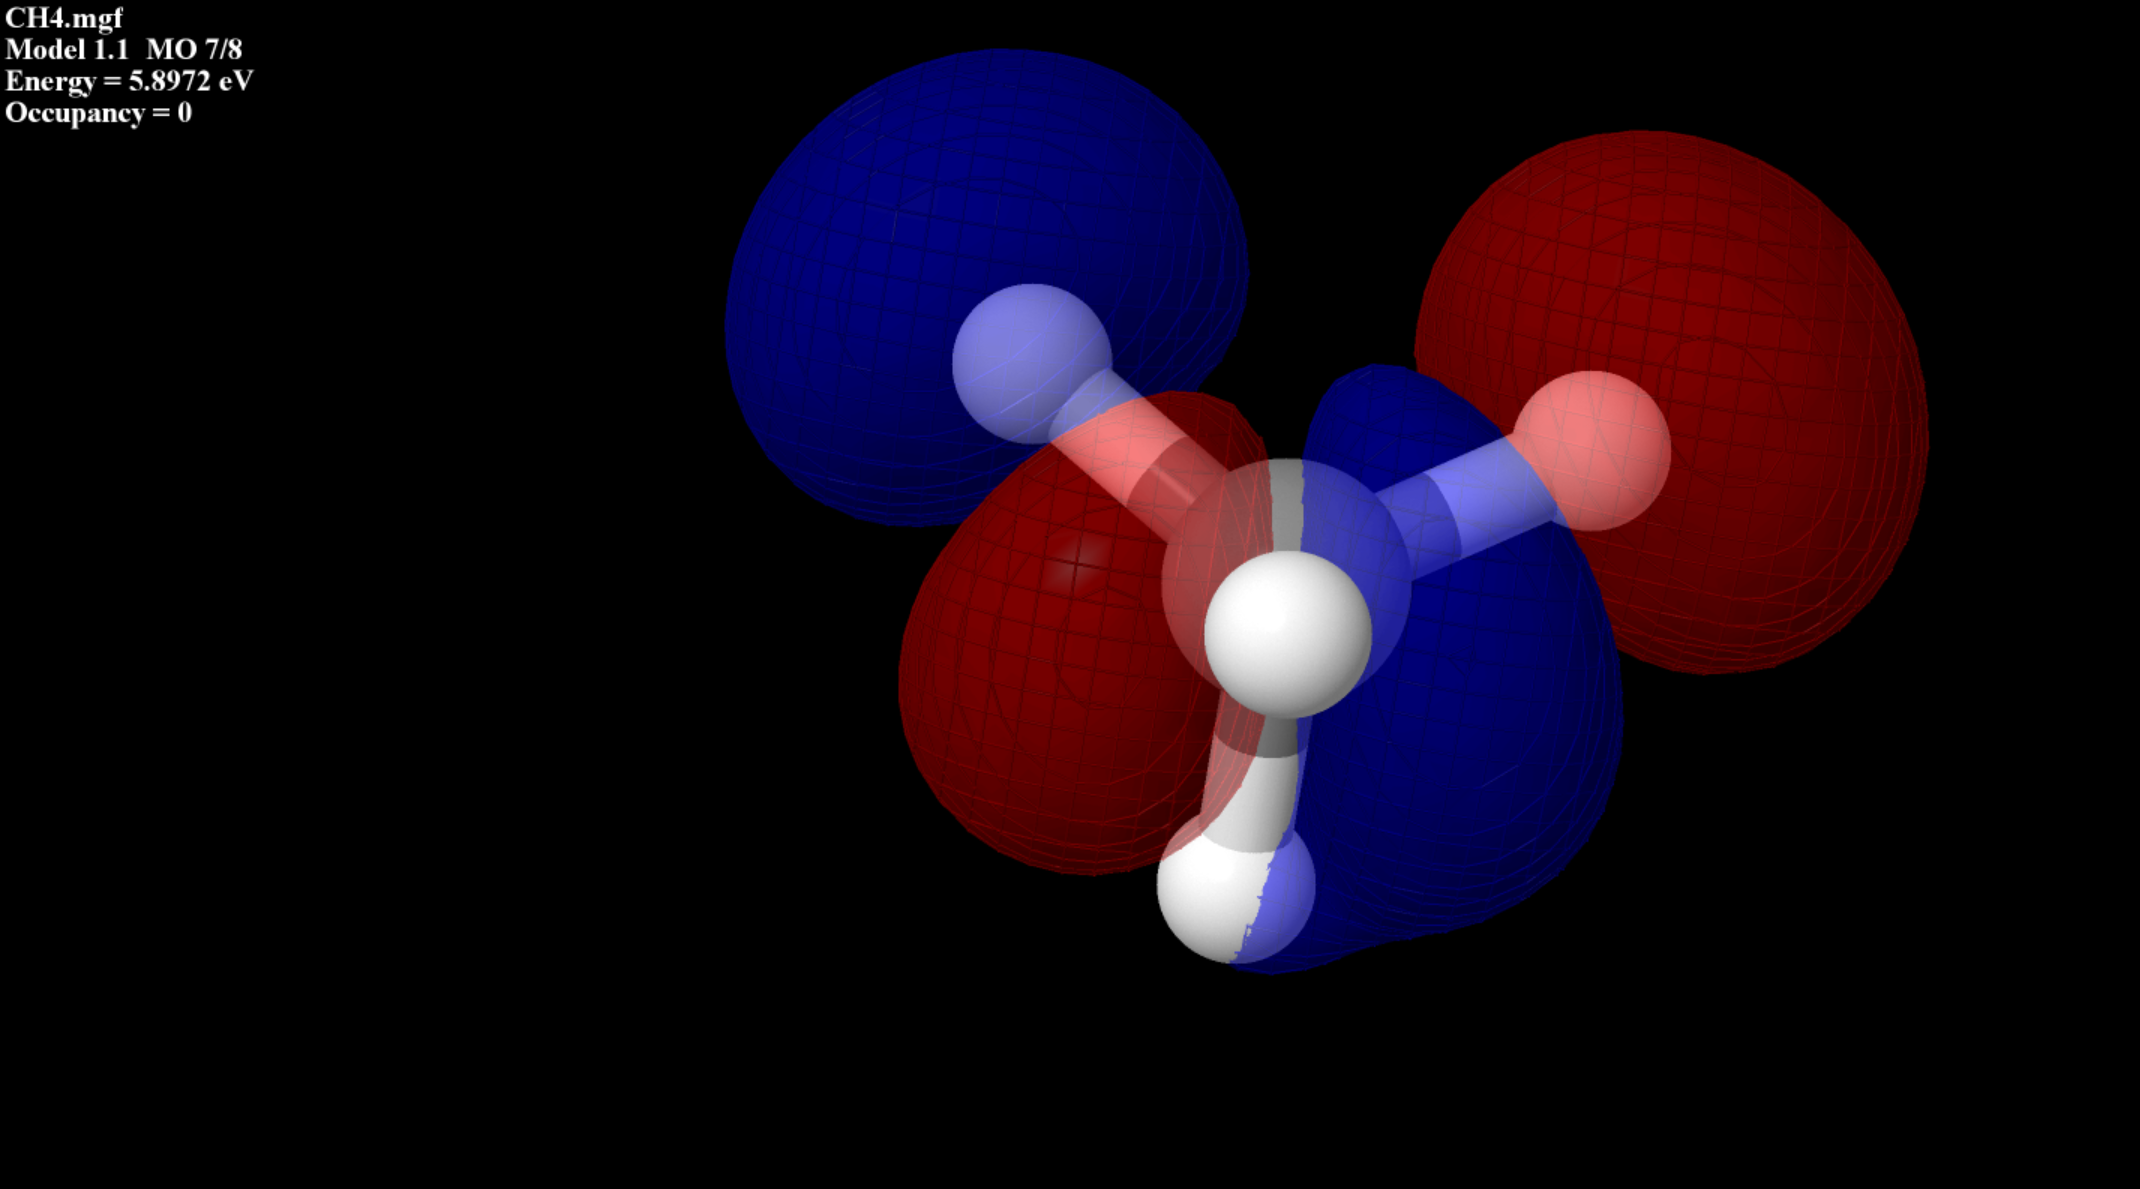
\includegraphics[width=\textwidth]{images-OM/MO 7 - CH4.png}
        \caption{OM 7}
        \label{fig:}
    \end{subfigure}
    \hspace{0.5cm}
    \begin{subfigure}{0.48\textwidth}
        \centering
        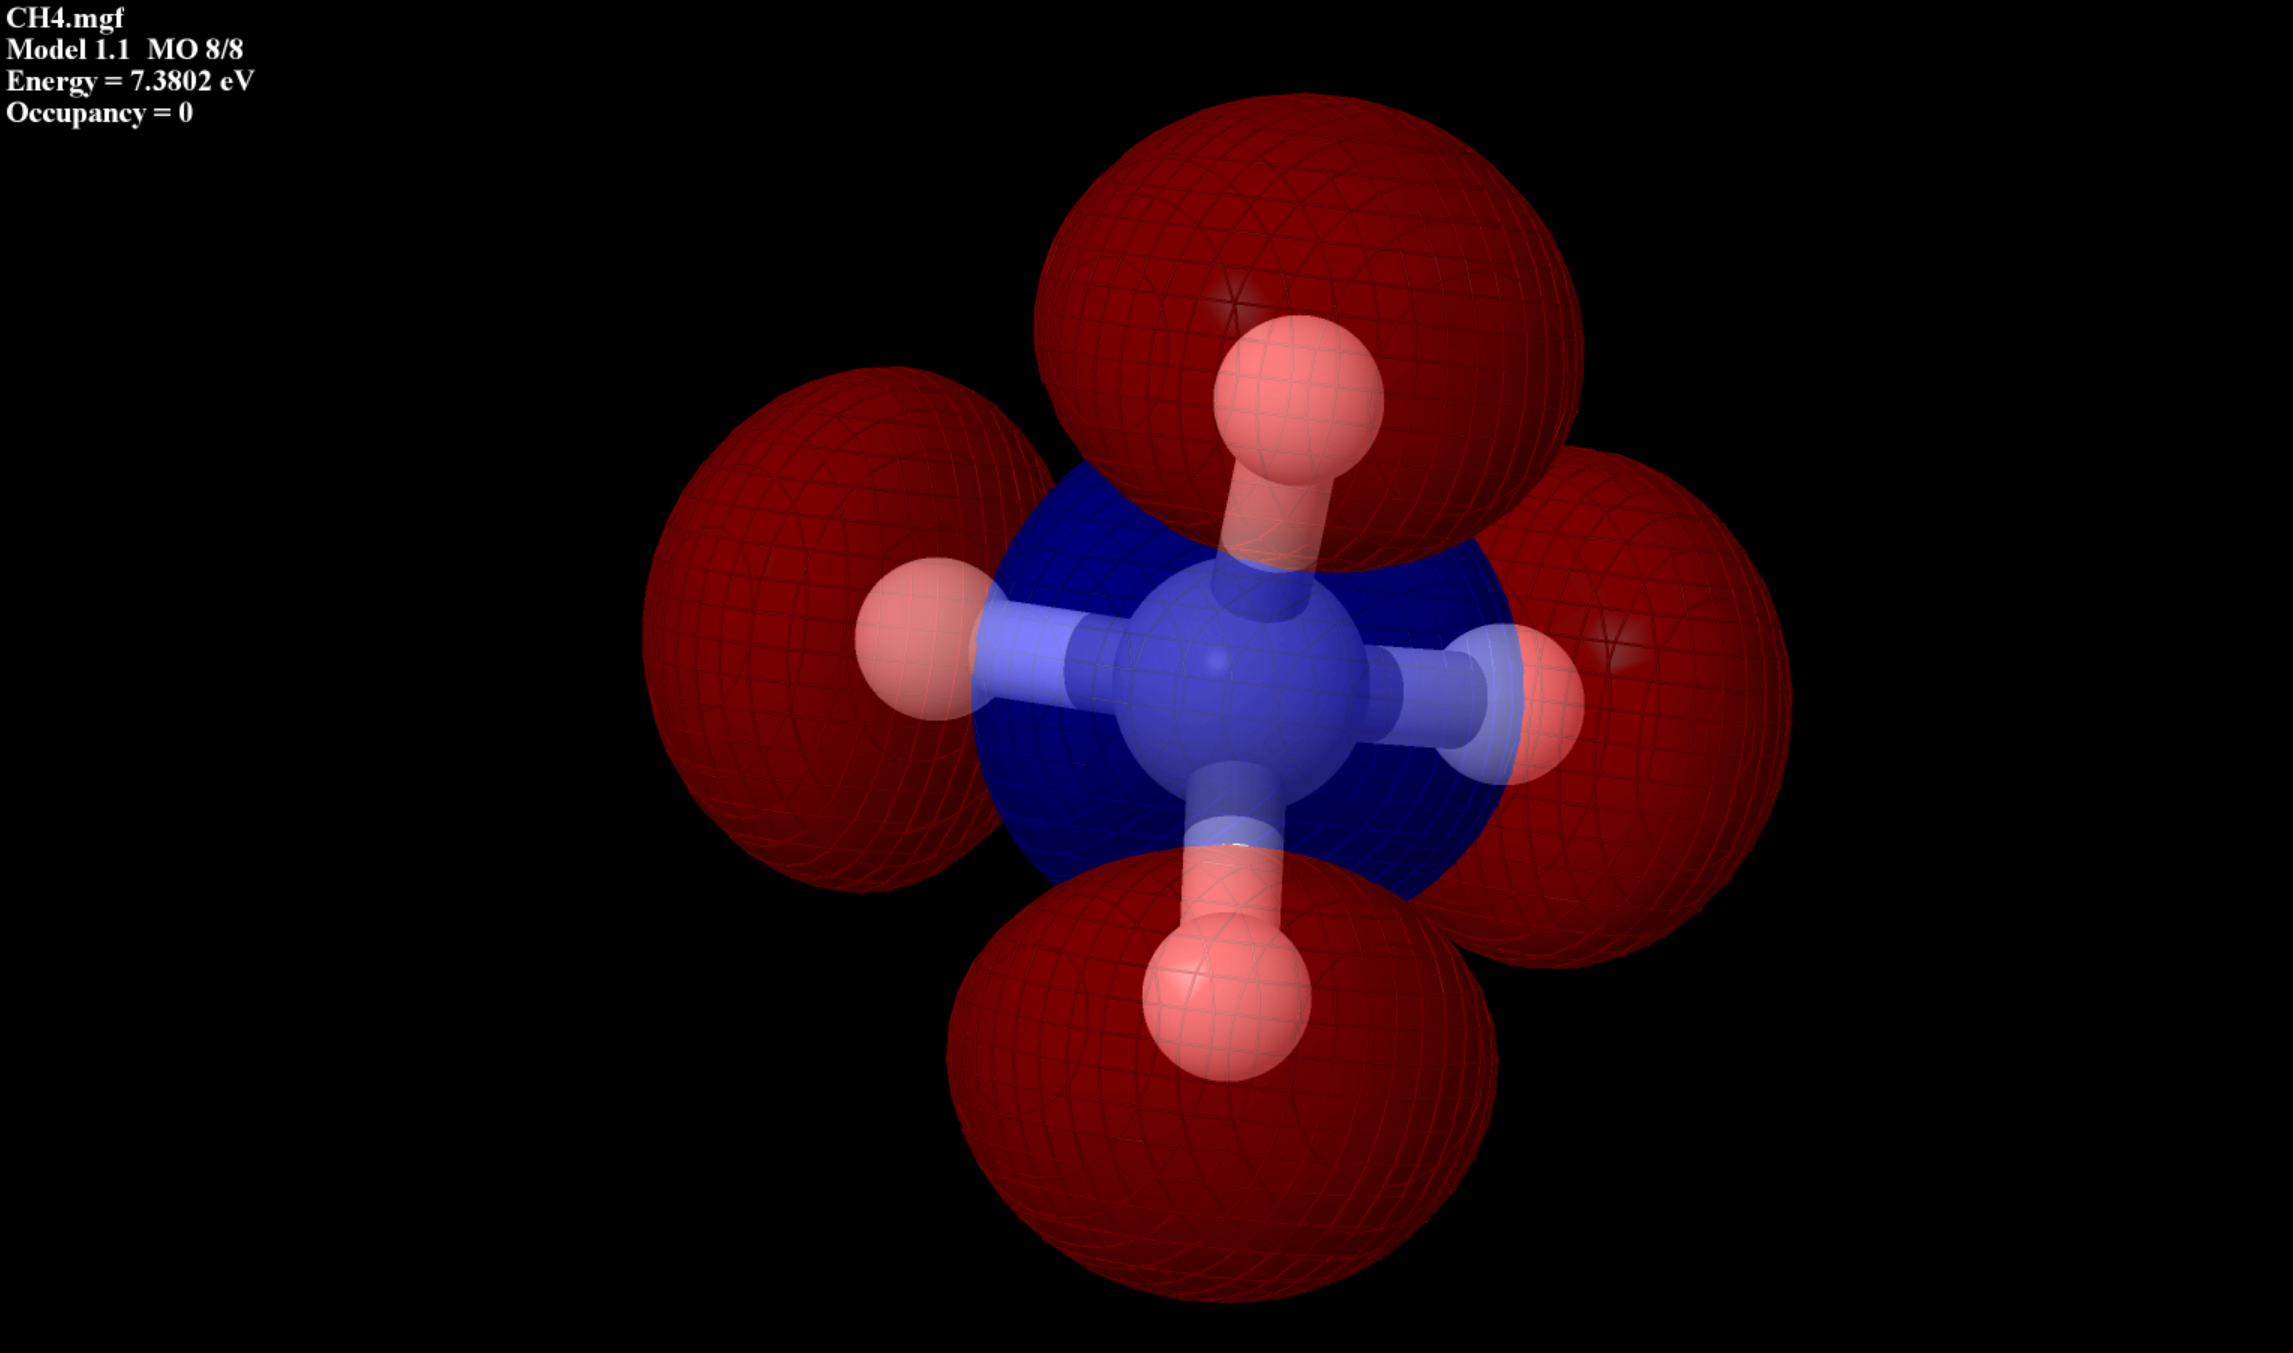
\includegraphics[width=\textwidth]{images-OM/MO 8 - CH4.png}
        \caption{OM 8}
        \label{fig:}
    \end{subfigure}
    \caption{Visualisation des quatres OM non occupées (donc non modifiées)}
\end{figure}

Voici les quatre autres OM de CH$_4$ non occupées par des électrons dans l'état fondamental, d'où le fait qu'elles soient restées intactes après utilisation du programme. Cela nous conforte également dans l'idée que le programme fonctionne correctement (en tout cas pour le méthane). \\

\dashuline{Critère de réussite de la localisation d'orbitales du programme :} \\

Finalement, il est intéressant de pouvoir vérifier sans même avoir besoin de visualiser les orbitales unes par unes (ce qui peut être long pour des grosses molécules et lorsque la quantité augmente) que la localisation des orbitales s'est bien faite sur chaque liaison de la molécule. Cette vérification est donc bien possible mais plusieurs conditions sont nécessaires, par ordre de priorité. \\

Il faut donc vérifier que l'on a UNIQUEMENT des contributions d'orbitales atomiques provenant des \textbf{deux atomes concernés} dans la liaison parmi toutes les orbitales mises en jeu dans l'OM (les autres doivent être négligeables, au minimum de l'ordre de 10$^{-2}$). Prenons le cas de CH$_4$, il faut donc une ou plusieurs OA de C (2s, 2p$_x$ et 2p$_y$ par exemple) et une OA d'un des H, tous les autres coefficients doivent être négligeables, il ne faut surtout pas de contribution d'OA d'autres hydrogènes sinon l'OM sera considérée comme non localisée.

De plus, il est nécessaire de \textbf{vérifier la normalisation au sein de chaque OM}. Donc pour le cas de CH$_4$, que pour chaque OM \( \sum_{i=1}^{8} C_i^{2} = 1\), ce que le programme fait automatiquement mais il n'interrompt pas le calcul si elle n'est pas vérifiée.

En effet, lors de notre court test avec NH$_3$, la normalisation n'était pas vérifiée sur la 4$^{\text{ème}}$ OM (tous les coefs étaient nuls ...), ce qui induisait que malgré le fait que les trois autres OM occupées respectaient les deux règles, la localisation n'avait sûrement pas été fructueuse. Finalement, après visualisation les lobes n'étaient effectivement pas bien localisés sur les liaisons.

%Le programme vérifie la normalisation au sein de chaque OM puis entre chaques OM ? 

%POUR BIEN VISUALISER SUR JMOL on tape la commande 
%mo fill
%mo translucent 0.5
\section{Conclusion \& Perspectives}

Globalement, l'application de notre programme sur le méthane est plutôt fructueuse puisque les lobes des OM pleines localisées sont cohérents et bien placés sur les liaisons. On retrouve bien des OM résultant d'un recouvrement d’orbitales hybrides sp$^3$. Les quatre autres OM non occupées n'ont pas été touchées, ce qui est normal mais heureux.

Cependant, nous avons été contraints de changer légèrement la méthode d'approche du programme préconisé par la publication puisque celle-ci considérait une minimisation des valeurs propres. Mais il s'est avéré plus pratique de partir sur une maximisation, et donc de considérer une Matrice R avec les données des deux atomes formant la liaison et non l'inverse. \\

Finalement, le sujet étant assez complexe, la lecture de la publication et la compréhension des objectifs du programme nous a pris plus de temps que prévu. Malgré cela, nous avons testé le programme sur la molécule NH$_3$ mais à cause du doublet non liant de N, un problème de dégénérescence des valeurs propres s'est posé. Par manque de temps, nous n'avons pas plus considéré le cas de NH$_3$, ce qui aurait été intéressant puisque les auteurs de la publication avaient étudié son cas et également expliqué le problème de dégénérescence.


%\newpage (surtout utile pour publi en double colonnes)
\nocite{*} 
\printbibliography 
\section{Annexe}
% METTRE TOUT LE CODE !!

\dashuline{Voici le code du programme, codé en C :}
\dashuline{Main.c :}
\begin{C}
#include <stdlib.h>
#include <stdio.h>
#include <math.h>
#include <string.h>

#include <limits.h>
#include <sys/stat.h>
#include <errno.h>
#include <unistd.h>


#include "../includes/matrice.h"
#include "../includes/luMethod.h"
#include "../includes/gestionfichier.h"

int main(int argc, const char * argv[]) {
    
    char cwd[PATH_MAX];
    if (getcwd(cwd, sizeof cwd)) printf("CWD = %s\n", cwd);
    
    Matrice E;
    
    int* aoParAtome;
    int natoms;
    if(lirefichier("data/CH4.mgf", &E, &aoParAtome, &natoms)!=1){
        printf("Erreur dans la lecture du fichier");
        exit(EXIT_FAILURE);
    }
    printf("Voici la matrice E comme elle est toute belle : \n");
    afficheMatrice(E);
    printf("On a : %d atomes ! \n", natoms);
    
    int nAO = E.n;
    
    //On stockera nos différents E_prime = EXij ici :
    int nTE_prime = natoms*(natoms-1)/2;
    Matrice TE_prime[nTE_prime];
    
    
    for (int i = 0; i < natoms; i++) {
        printf("Atome %d → %d AO\n", i+1, aoParAtome[i]);
    }
    int compteur = 0;
    //C'est parti pour traiter chaque liaison une par une
    for (int i = 0; i < natoms; i++) {
        for (int j = i + 1; j < natoms; j++) { //Liaison entre i et j
            printf("Itération %d\n", compteur);
            compteur++;
            //Choisissons les lignes à éliminer
            int *tokeep = malloc(nAO * sizeof(int));
            
            //Puis on assigne les lignes de la matrice E idoine dans R :
            int compte = 0;
            for(int k = 0; k<natoms; k++)
            {
                for(int l = k; l - k <aoParAtome[k]; l++)
                {
                    //Si c'est un atome concerné par la liaison : CA DEGAGE
                    if(k== i || k == j) tokeep[compte] = 0;
                    else tokeep[compte] = 1;
                    compte++;
                    //printf("l = %d k = %d AoPA = %d l+k= %d  :: \n", l, k, aoParAtome[k], l+k);
                }
                
            }
            //for(int w = 0; w<nAO; w++){printf("%d  ", tokeep[w]);}
            //printf("\nON CHANGE DE LIAISON \n");
            
            //Maintenant qu'on a cette p- sacré liste, on crée notre variable R à partir de E.
            //Calculons la taille de R..
            int nRRow = nAO - aoParAtome[i] - aoParAtome[j];
            Matrice R = createMatrice(nRRow, nAO);
            
            //Pour chaque ligne, si l'AO contribue à la liason : ligne de 0, sinon : ligne de R.
            int compteR = 0;
            for(int i=0; i<nAO; i++){
                if(tokeep[i]){
                    for(int j =0; j<nAO; j++){
                        R.data[compteR][j] = E.data[i][j];
                    }
                    compteR++;
            }
        }
            
        //On calcule ensuite TRR (R^T*R)
        Matrice TR = transpose(R);
        Matrice TRR = produit(TR, R);
        //Ensuite on diagonalise la matrice
        Matrice VectPR = createMatrice(nAO, nAO);
        vpJacobi(TRR, VectPR);
        
        //Matrice colonne des VALEURS propres de R
        Matrice VPdeR = vpDiag(TRR);
        int position;
        double vp = minVP(VPdeR, &position);
        printf("Valeur propre : %g\n", vp);
        //On récupère le vecteur propre X correspondant à cette position
        Matrice X = getCol(VectPR, position);
        //On multiple E par ce vecteur colonne pour obtenir Li
        Matrice Li = produit(E, X);
        TE_prime[compteur] = copieMatrice(Li);
    }
}

//NORMALEMENT on a toute nos matrice Eprime, faisons en la moyenne !
Matrice EPrime = meanMatrices(TE_prime, nTE_prime);
printf("La sainte Matrice E' : \n");
afficheMatrice(EPrime);
int res = ecrire_orbital_replaced("data/CH4.mgf", "output/CH4.mgf", &EPrime, nAO);
printf("Conclusion du code : %d \n", res);
return EXIT_SUCCESS;
\end{C}

\dashuline{matrice.c :}
\begin{C}
#include <stdlib.h>
#include <stdio.h>
#include <math.h>
#include "matrice.h"

#define TOL 1e-12

void jacobi(double **a, double **b, int n);

//M[i] = Pointeur de la ligne
Matrice createMatrice(int n, int m) //LiCo //Crée une matrice de taille m*n sans valeur particulière
{
    Matrice matrice;
    matrice.n = n; //ligne
    matrice.m = m; //colonne
    //Allocation du tableau de pointeur
    matrice.data = malloc(n * sizeof(double));
    if(!matrice.data)
    {
        printf("Echec de l'allocation mémoire lors de la création \n");
        exit(EXIT_FAILURE);
    }
    
    //Allocation des lignes
    for( int i = 0; i<n ; i++)
    {
        matrice.data[i] = malloc(m * sizeof(double));
        if(!matrice.data[i])
        {
            printf("Echec de l'allocation mémoire lors de la création \n");
            exit(EXIT_FAILURE);
        }
        for(int j=0; j<m; j++)
        {
            matrice.data[i][j] = 0;
        }
    }
    
    return matrice;
}

void freeMatrice(Matrice *M) {
    if (!M || !M->data) return;
    
    // libérer chaque ligne
    for (int i = 0; i < M->n; i++) {
        free(M->data[i]);
    }
    
    // libérer le tableau de pointeurs
    free(M->data);
    
    // mettre les champs à zéro pour éviter les "dangling pointers"
    M->data = NULL;
    M->n = 0;
    M->m = 0;
}

Matrice copieMatrice(Matrice M){
    Matrice res = createMatrice(M.n, M.m);
    for (int i=0; i<M.n; i++) {
        for (int j=0; j<M.m; j++) {
            res.data[i][j] = M.data[i][j];
        }
    }
    return res;
}

void afficheMatrice(Matrice mat) //Affiche la matrice
{
    if(mat.n < 0 || mat.m < 0){
        printf("Affichage matrice impossible\n");
        exit(EXIT_FAILURE);
    }
    for(int i = 0; i<mat.n; i++)
    {
        for(int j=0; j<mat.m;j++)
        {
            printf("%10.2g", mat.data[i][j]);
        }
        printf("\n");
    }
}

//Génére une matrice de test où chaque coeff = id_coeff
void testMatrice(Matrice M)
{
    int k = 0;
    for(int i=0; i<M.n; i++)
    {
        for(int j=0; j<M.m; j++)
        {
            M.data[i][j] = k;
            k++;
        }
    }
}

//Crée la matrice transposé
Matrice transpose(Matrice M)
{
    double a = M.n, b = M.m;
    //Dans M : 0<i<a ; 0<j<b
    //Dans MT : 0<i<b; 0<j<a
    Matrice MT = createMatrice(b, a);
    for(int i=0; i<a; i++)
    {
        for(int j=0; j<b; j++)
        {
            MT.data[j][i] = M.data[i][j];
        }
    }
    
    return MT;
}

//Crée le produit de deux matrices
Matrice produit(Matrice M, Matrice N)
{
    if(M.m != N.n)
    {
        printf("Produit Matriciel invalide !! \n");
        exit(EXIT_FAILURE);
    }
    int n_somme = M.m;
    Matrice res = createMatrice(M.n, N.m);
    for(int i=0; i<res.n; i++)
    {
        for(int j=0; j<res.m; j++)
        {
            double coeff = 0;
            for(int k = 0; k<n_somme; k++)
            {
                coeff += M.data[i][k]*N.data[k][j];
            }
            res.data[i][j] = coeff;
        }
    }
    return res;
}

void pScaMat(Matrice M, double a){
    for(int i=0; i<M.n; i++)
    {
        for(int j=0; j<M.m; j++)
        {
            M.data[i][j] = a*M.data[i][j];
        }
    }
}

double pScalaire(Matrice X)
{
    if(X.m != 1)
    {
        printf("Pas un vecteur colonne !!! \n");
        exit(EXIT_FAILURE);
    }
    Matrice TX = transpose(X);
    return produit(X, TX).data[0][0];
    
}
//Addition M + aN
Matrice addMat(Matrice M, Matrice N, double a)
{
    if(M.n != N.n || M.m != N.m)
    {
        printf("Addition entre deux matrices de tailles différentes !! \n");
        exit(EXIT_FAILURE);
    }
    int n = M.n, m = M.m;
    Matrice res = createMatrice(n, m);
    
    for(int i=0; i<n;i++)
    {
        for(int j=0; j<m; j++)
        {
            res.data[i][j] = M.data[i][j] + a*N.data[i][j];
        }
    }
    return res;
}

double norme(Matrice M)
{
    return sqrt(pScalaire(M));
}

//Génère une matrice identité de taille n
Matrice Identite(int n)
{
    Matrice I = createMatrice(n, n);
    for(int i=0;i<n;i++)
    {
        for(int j=0; j<n; j++)
        {
            I.data[i][j] = i == j ? 1 : 0;
        }
    }
    
    return I;
}

//Donne un vecteur colonne des valeurs propre d'une matrice diagonale
Matrice vpDiag(Matrice D)
{
    if(D.n != D.m){
        printf("Matrice diagonale non carrée");
        exit(EXIT_FAILURE);
    }
    Matrice res = createMatrice(D.n, 1);
    for(int i=0; i<D.n; i++){
        res.data[i][0] = D.data[i][i];
    }
    return res;
}


double minVP(Matrice colVP, int *pos_out){
    if(colVP.m != 1){
        printf("Pas une matrice colonne");
        exit(EXIT_FAILURE);
    }
    double min = colVP.data[0][0];
    double pos = 0;
    for(int i=0; i<colVP.n; i++){
        if(fabs(colVP.data[i][0]) < fabs(min)) {
            min = colVP.data[i][0];
            pos = i;
        }
    }
    
    if(pos_out) *pos_out = pos;
    return min;
}

Matrice getCol(Matrice M, int pos){
    if(pos>= M.m){
        printf("Postion mauvaise");
        exit(EXIT_FAILURE);
    }
    
    Matrice res = createMatrice(M.m, 1);
    
    for (int i=0; i<M.n; i++) {
        res.data[i][0] = M.data[i][0];
    }
    return res;
}

//Compatibilité Structure Matrice <-> Fonction Jacobi des TP 1A
void vpJacobi(Matrice a, Matrice b)
{
    if(a.n != a.m || b.n != b.m || a.n != b.n)
    {
        printf("Entrée invalide pour Jacobi");
        exit(EXIT_FAILURE);
    }
    jacobi(a.data, b.data, a.n);
}

//Moyenne arithmétique d'une liste de matrice
Matrice meanMatrices(const Matrice *list, int count) {
    if (!list || count <= 0) {
        // signal d'erreur : matrice vide (pas d'allocation)
        Matrice err = {0, 0, NULL};
        return err;
    }

    const int n = list[0].n;
    const int m = list[0].m;

    // Vérification des dimensions
    for (int k = 0; k < count; k++) {
        Matrice justpourvoir = list[k];
        if (list[k].n != n || list[k].m != m || list[k].data == NULL) {
            Matrice err = {0, 0, NULL};
            return err;
        }
    }

    // Somme : S = list[0] + list[1] + ... + list[count-1]
    Matrice S = copieMatrice(list[0]);      // S = list[0]
    for (int k = 1; k < count; k++) {
        Matrice tmp = addMat(S, list[k], 1.0); // tmp = S + 1.0 * list[k]
        freeMatrice(&S);
        S = tmp;
    }

    // Moyenne : S *= 1/count (in place)
    pScaMat(S, 1.0 / (double)count);
    return S; // À libérer par l'appelant avec freeMatrice(&S)
}

//Donne la matrice des vecteurs propres
//OUTPUT : a : matrice diagonalisé b : matrice des vecteurs propres
//a = matrice carré; b = vecteur; n = taille
void jacobi(double **a, double **b, int n)
{
    int i,j,k,l;
    double M,alpha,t,h,c,s,r,u,v;
    int iter=0;
    
    for (i=0;i<n;i++)
    { for (j=0;j<n;j++) b[i][j]=0;
        b[i][i]=1;
    }
    
    do {
        M=0;
        for (i=0;i<n-1;i++)
            for (j=i+1;j<n;j++)
                if (fabs(a[i][j])>M) {
                    k=i;
                    l=j;
                    M=fabs(a[i][j]);
                }
        
        if (M<TOL) break;
        iter++;
        alpha=0.5*(a[l][l]-a[k][k])/a[k][l];
        t=sqrt(1+alpha*alpha);
        if (alpha<0)
            t=-t;
        t-=alpha;
        h=t*a[k][l];
        c=1/sqrt(1+t*t);
        s=t*c;
        r=s/(1+c);
        for (j=0;j<n;j++) {
            u=b[j][k];
            v=b[j][l];
            b[j][k]-=s*(v+r*u);
            b[j][l]+=s*(u-r*v);
            if (j!=k && j!=l) {
                u=a[k][j];
                v=a[l][j];
                a[k][j]-=s*(v+r*u);
                a[l][j]+=s*(u-r*v);
                a[j][k]=a[k][j];
                a[j][l]=a[l][j];
            }
        }
        a[k][k]-=h;
        a[l][l]+=h;
        a[k][l]=a[l][k]=0;
    } while (M>TOL && iter<1000);
    }
\end{C}
\dashuline{matrice.h :}
\begin{C}
#ifndef MATRICE_H
#define MATRICE_H

//Définition d'une Matrice
typedef struct {
    int n;
    int m;
    double** data;
} Matrice;

Matrice createMatrice(int n, int m);
void freeMatrice(Matrice *M);
Matrice copieMatrice(Matrice M);
void pScaMat(Matrice M, double a);
double pScalaire(Matrice X);
Matrice addMat(Matrice M, Matrice N, double a);
double norme(Matrice M);
Matrice Identite(int n);
void afficheMatrice(Matrice mat);
void testMatrice(Matrice M);
Matrice transpose(Matrice M);
Matrice produit(Matrice M, Matrice N);
Matrice vpDiag(Matrice D);
double minVP(Matrice colVP, int *pos_out);
Matrice getCol(Matrice M, int pos);
Matrice meanMatrices(const Matrice *list, int count);
void vpJacobi(Matrice a, Matrice b);

#endif
\end{C}

\dashuline{luMethod.c :}
\begin{C}
#include <stdlib.h>
#include <stdio.h>
#include <math.h>

#include "matrice.h"
#include "luMethod.h"

/* INPUT: A - array of pointers to rows of a square matrix having dimension N
 *        Tol - small tolerance number to detect failure when the matrix is near degenerate
 * OUTPUT: Matrix A is changed, it contains a copy of both matrices L-E and U as A=(L-E)+U such that P*A=L*U.
 *        The permutation matrix is not stored as a matrix, but in an integer vector P of size N+1
 *        containing column indexes where the permutation matrix has "1". The last element P[N]=S+N,
 *        where S is the number of row exchanges needed for determinant computation, det(P)=(-1)^S
 */
int LUPDecompose(Matrice A, double Tol, int *P) {
    if(A.n != A.m)
    {
        printf("Décomposition LU sur une matrice non carré !!!\n");
        exit(EXIT_FAILURE);
    }

    int i, j, k, imax;
    int N = A.n;
    double maxA, *ptr, absA;

    for (i = 0; i <= N; i++)
        P[i] = i; //Unit permutation matrix, P[N] initialized with N

    for (i = 0; i < N; i++) {
        maxA = 0.0;
        imax = i;

        for (k = i; k < N; k++)
            if ((absA = fabs(A.data[k][i])) > maxA) {
                maxA = absA;
                imax = k;
            }

        if (maxA < Tol) return 0; //failure, matrix is degenerate

        if (imax != i) {
            //pivoting P
            j = P[i];
            P[i] = P[imax];
            P[imax] = j;

            //pivoting rows of A
            ptr = A.data[i];
            A.data[i] = A.data[imax];
            A.data[imax] = ptr;

            //counting pivots starting from N (for determinant)
            P[N]++;
        }

        for (j = i + 1; j < N; j++) {
            A.data[j][i] /= A.data[i][i];

            for (k = i + 1; k < N; k++)
                A.data[j][k] -= A.data[j][i] * A.data[i][k];
        }
    }
    
    return 1;  //decomposition done
}


/* INPUT: A,P filled in LUPDecompose; N - dimension
 * OUTPUT: IA is the inverse of the initial matrix
 */
Matrice LUPInvert(Matrice A, int *P) {
    
    Matrice IA = copieMatrice(A);
    
    if(A.n != A.m)
    {
        printf("Inversion LU sur une matrice non carré !!!\n");
        exit(EXIT_FAILURE);
    }
    int N = A.n;
  
    for (int j = 0; j < N; j++) {
        for (int i = 0; i < N; i++) {
            IA.data[i][j] = P[i] == j ? 1.0 : 0.0;

            for (int k = 0; k < i; k++)
                IA.data[i][j] -= A.data[i][k] * IA.data[k][j];
        }

        for (int i = N - 1; i >= 0; i--) {
            for (int k = i + 1; k < N; k++)
                IA.data[i][j] -= A.data[i][k] * IA.data[k][j];

            IA.data[i][j] /= A.data[i][i];
        }
    }
    
    return IA;
}

/* INPUT: A,P filled in LUPDecompose; N - dimension.
 * OUTPUT: Function returns the determinant of the initial matrix
 */
double LUPDeterminant(Matrice A, int *P) {
    
    if(A.n != A.m)
    {
        printf("Calcul de determinant LU sur une matrice non carré !!!\n");
        exit(EXIT_FAILURE);
    }
    int N = A.n;

    double det = A.data[0][0];

    for (int i = 1; i < N; i++)
        det *= A.data[i][i];

    return (P[N] - N) % 2 == 0 ? det : -det;
}
\end{C}

\dashuline{luMethod.h :}
\begin{C}
#ifndef LUMETHOD_H
#define LUMETHOD_H

#include "matrice.h"

int LUPDecompose(Matrice A, double Tol, int *P);
Matrice LUPInvert(Matrice A, int *P);
double LUPDeterminant(Matrice A, int *P);

#endif
\end{C}

\dashuline{gestionfichier.c :}
\begin{C}
#include <stdlib.h>
#include <stdio.h>
#include <math.h>
#include <string.h>
#include <ctype.h>

#include "gestionfichier.h"
#include "matrice.h"

void sauteLigne(FILE *f);
int ao_count_for_Z(int Z);

int lirefichier(const char *path, Matrice *E,int **aoParAtome, int *natoms_out)
{
    FILE *f;
    
    f=fopen(path,"r");
    if (f==0) {printf("Problème d'ouverture du fichier !\n"); exit(EXIT_FAILURE);}
    //On veut le nombre d'atomes
    int natoms = 0;
    if (fscanf(f, " %d", &natoms) != 1) {   // " %d" saute les espaces initiaux
        fprintf(stderr, "Impossible de lire le nombre d'atomes en tête de fichier.\n");
        fclose(f);
        return 2;
    }
    printf("Nombre d'atomes = %d\n", natoms);
    //Sautons une ligne
    sauteLigne(f);
    
    //C'est l'occasion d'allouer le tableau :)
    if (aoParAtome) {
        *aoParAtome = malloc(natoms * sizeof(int));
        if (!*aoParAtome) { fclose(f); return -100; }
    }
    
    
    //On en déduit le nombre d'AO du système
    //Pour cela on prend trouve les éléments chimiques de chacun et on additionne selon la période.
    int nAO = 0;
    for(int i=0; i<natoms;i++)
    {
        int Z;
        //On récupère son numéro atomique
        if(fscanf(f, " %d %*lf %*lf %*lf %*lf", &Z) != 1){
            fprintf(stderr, "Ligne d'atome %d invalide.\n", i+1);
            fclose(f);
            exit(EXIT_FAILURE);
        }
        if(Z<3)//Période 1 -> 1 AO
        {
            nAO += 1;
            if (aoParAtome && *aoParAtome) (*aoParAtome)[i] = 1;
        }
        else if(Z==6 || Z==7 || Z==8 || Z==9)//Période 2 -> 4 AO
        {
            nAO += 4;
            if (aoParAtome && *aoParAtome) (*aoParAtome)[i] = 4;
        }
        else
        {
            printf("Numéro atomique trop lourd !");
            exit(EXIT_FAILURE);
        }
    }
    
    printf("Nombre Orbitale Atomique : %d \n", nAO);
    
    //Maitenant on prépare notre matrice E : E[OA][OM] (je suis trop hype)
    *E = createMatrice(nAO, nAO);
    
    //C'est parti pour chercher les nAO dans le fichier
    char line[4096];
    int count = 0;
    
    int i=0;
    
    while (fgets(line, sizeof line, f) && i<nAO) {
        // Tolère des espaces avant "ORBITAL"
        const char *p0 = line;
        while (*p0==' ' || *p0=='\t' || *p0=='\r') p0++;
        if (strncmp(line, " ORBITAL", 7) == 0) {
            // Récupérer l'énergie (eV) écrite après "ORBITAL"
            // Exemple de ligne : " ORBITAL 2" ou "ORBITAL 0"
            double ev = 0.0;
            const char *p = p0 + 7;             // après "ORBITAL"
            while (*p==' ' || *p=='\t') p++;    // espaces
            if (*p) {
                char *endp = NULL;
                // strtod accepte 2, 2.0, +2.3e-1, etc.
                double tmp = strtod(p, &endp);
                if (endp != p) ev = tmp;
            }
            if (ev_out) {
                ev_out->data[i][0] = ev; // stocke l’énergie de la MO i (en eV)
            }
            int got = 0;  // nb de doubles collectés pour cette orbitale
            
            // Lire des lignes suivantes et accumuler des doubles jusqu’à en avoir nAO
            while (got < nAO && fgets(line, sizeof line, f)) {
                char *p = line;
                while (*p && got < nAO) {
                    // sauter espaces
                    while (*p == ' ' || *p == '\t' || *p == '\r' || *p == '\n') p++;
                    if (!*p) break;
                    
                    char *endp;
                    double v = strtod(p, &endp);
                    if (endp == p) break; // rien de lisible sur ce reste de ligne
                    
                    E->data[got][i] = v;   // j = got
                    got++;
                    p = endp;
                }
            }
            
            if (got != nAO) {
                fprintf(stderr, "Erreur: orbitale %d incomplète (%d/%d coeffs lus).\n",
                        i+1, got, nAO);
                fclose(f);
                return 10;
            }
            i++;       // prochaine orbitale
            count++;   // compteur d’ORBITAL vues
        }
    }
    
    printf("Total ORBITAL: %d\n", count);
    *natoms_out = natoms;
    fclose(f);
    return 1;
}

// saute le reste de la ligne courante (jusqu’à et y compris '\n')
void sauteLigne(FILE *f) {
    int ch;
    while ((ch = fgetc(f)) != EOF && ch != '\n') {
        // on boucle tant qu’on n’a pas rencontré un retour ligne
    }
}

int ao_count_for_Z(int Z) {
    if (Z < 3) return 1;                       // H (He non utilisé ici)
    if (Z==6 || Z==7 || Z==8 || Z==9) return 4; // C, N, O, F
    return 0; // non géré ici
}

/* saute espaces initiaux (ne modifie pas la chaîne d'origine) */
static const char* lskip(const char *s) {
    while (*s == ' ' || *s == '\t' || *s == '\r') ++s;
    return s;
}

/* compte le nb de doubles lisibles dans 'line' (tolère D/d → E) ;
   renvoie aussi si la ligne contenait un 'D' */
static int count_doubles_in_line(const char *line, int *saw_D) {
    char tmp[4096];
    size_t L = strlen(line);
    if (L >= sizeof tmp) L = sizeof tmp - 1;
    memcpy(tmp, line, L); tmp[L] = '\0';

    int saw = 0;
    for (size_t i = 0; i < L; ++i) {
        if (tmp[i] == 'D' || tmp[i] == 'd') { tmp[i] = 'E'; saw = 1; }
    }
    if (saw_D) *saw_D |= saw;

    int count = 0;
    char *p = tmp;
    for (;;) {
        while (isspace((unsigned char)*p)) ++p;
        if (!*p) break;
        char *endp;
        (void)strtod(p, &endp);
        if (endp == p) break;
        ++count;
        p = endp;
    }
    return count;
}

/* imprime v dans buf, fmt %.12E, puis remplace E→D si use_D */
static void format_double_ED(char *buf, size_t bufsz, double v, int use_D) {
    snprintf(buf, bufsz, "%.12E", v);
    if (use_D) {
        for (char *p = buf; *p; ++p) if (*p == 'E') *p = 'D';
    }
}

/* --- fonction principale --- */

int ecrire_orbital_replaced(const char *in_path, const char *out_path,const Matrice *E, int nAO)
{
    if (!in_path || !out_path || !E || nAO <= 0) return -1;

    FILE *in = fopen(in_path, "r");
    if (!in) return -2;

    FILE *out = fopen(out_path, "w");
    if (!out) { fclose(in); return -3; }

    char line[4096];
    int mo = 0; /* index du bloc ORBITAL courant (0..nAO-1) */

    while (fgets(line, sizeof line, in)) {
        const char *q = lskip(line);

        /* Si ce n'est pas un début de bloc ORBITAL, recopier tel quel */
        if (strncmp(q, "ORBITAL", 7) != 0) {
            fputs(line, out);
            continue;
        }

        /* Début de bloc ORBITAL : recopier l'en-tête */
        fputs(line, out);

        /* On va consommer dans l'entrée les lignes suivantes jusqu'à lire nAO nombres.
           Pour chaque ligne de nombres source (k nombres), on écrit k nombres
           pris dans E->data[oa][mo], en gardant l'indentation initiale. */
        if (mo >= nAO) {
            /* Plus de colonnes disponibles : on passe à travers sans remplacer */
            continue;
        }

        int got = 0;           /* nb de coeffs écrits pour cette ORBITAL */
        int prefer_D = 0;      /* si la première ligne numérique source utilise D, on l'imite */

        while (got < nAO && fgets(line, sizeof line, in)) {
            /* détecter indentation de la ligne source */
            size_t indent = 0;
            while (line[indent] == ' ' || line[indent] == '\t') ++indent;

            /* combien de nombres sur cette ligne ? */
            int k = count_doubles_in_line(line, &prefer_D);

            if (k == 0) {
                /* ligne sans nombres (vide/commentaire) : recopier telle quelle */
                fputs(line, out);
                continue;
            }

            /* écrire une ligne avec le même nombre de nombres (k), depuis E */
            if (indent > 0) fwrite(line, 1, indent, out); /* réécrit juste l'indentation */

            for (int t = 0; t < k && got < nAO; ++t, ++got) {
                char numbuf[64];
                
                // Vérifs défensives
                if (!E)            { fprintf(stderr,"E NULL\n"); exit(EXIT_FAILURE); }
                if (!E->data)      { fprintf(stderr,"E->data NULL\n"); exit(EXIT_FAILURE); }
                if (got < 0 || got >= nAO) { fprintf(stderr,"got=%d hors [0,%d)\n", got, nAO); exit(EXIT_FAILURE); }
                if (mo  < 0 || mo  >= nAO) { fprintf(stderr,"mo=%d hors [0,%d)\n",  mo,  nAO); exit(EXIT_FAILURE); }
                if (!E->data[got]) { fprintf(stderr,"E->data[%d] NULL\n", got); exit(EXIT_FAILURE); }
                
                format_double_ED(numbuf, sizeof numbuf, E->data[got][mo], prefer_D);
                if (t > 0) fputc(' ', out);
                fputs(numbuf, out);
            }
            fputc('\n', out);

            /* Si la ligne source contenait plus de nombres que nécessaire (rare),
               on ignore l'excédent, car on s'arrête quand got==nAO. */
            if (got >= nAO) break;
        }

        ++mo; /* bloc ORBITAL suivant */
    }

    fclose(in);
    fclose(out);
    return 0;
}
\end{C}

\dashuline{gestionfichier.h :}
\begin{C}
#ifndef GESTIONFICHIER_H
#define GESTIONFICHIER_H

#include "matrice.h"

int lirefichier(const char *path, Matrice *E, int **aoParAtome, int *natoms_out);
int ecrire_orbital_replaced(const char *in_path, const char *out_path,const Matrice *E, int nAO);

#endif
\end{C}

%\dashuline{Voici les fichiers Entrée et Sortie MGF pour CH$_4$ :}
\begin{figure}[H]
    \centering
    \begin{subfigure}{0.49\textwidth}
    \centering
    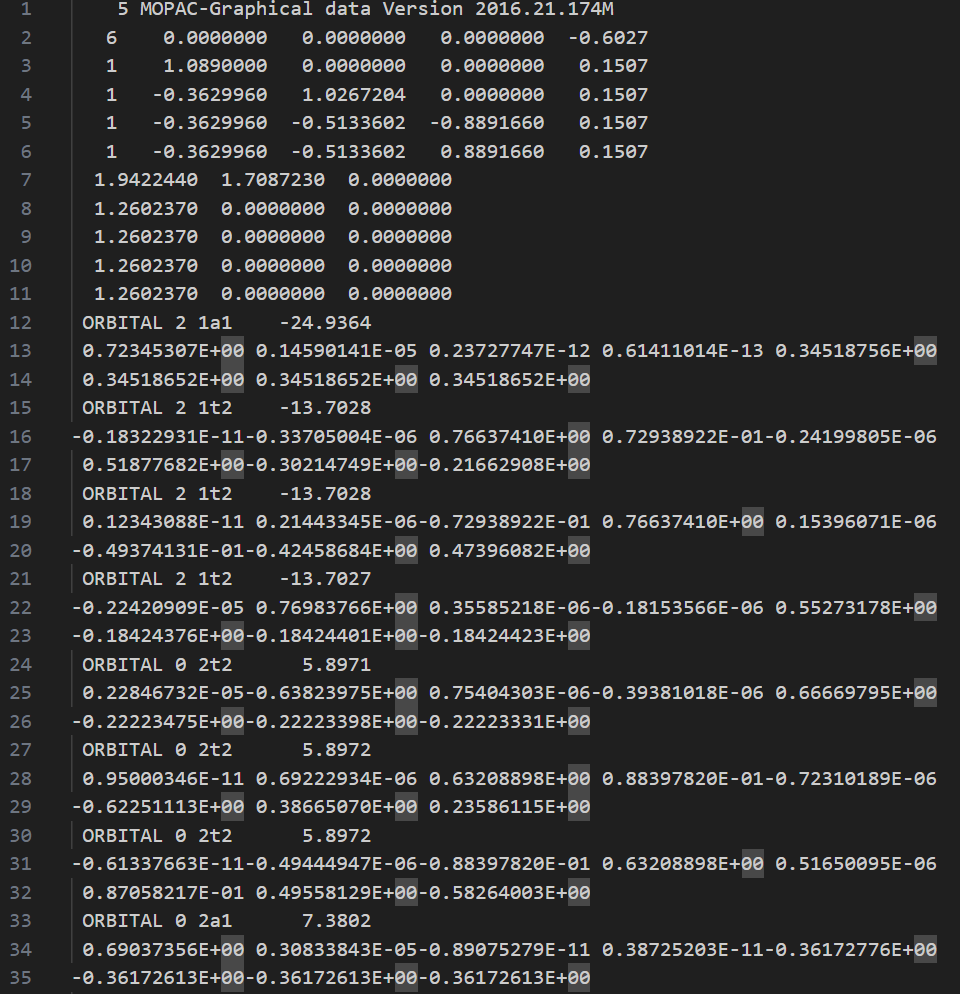
\includegraphics[width=\linewidth]{images autres/img_CH4_mgf.png}
    \caption{CH$_4$.mgf}       
    \end{subfigure}
       \hspace{0.1cm}
    \begin{subfigure}{0.49\textwidth}
    \centering
    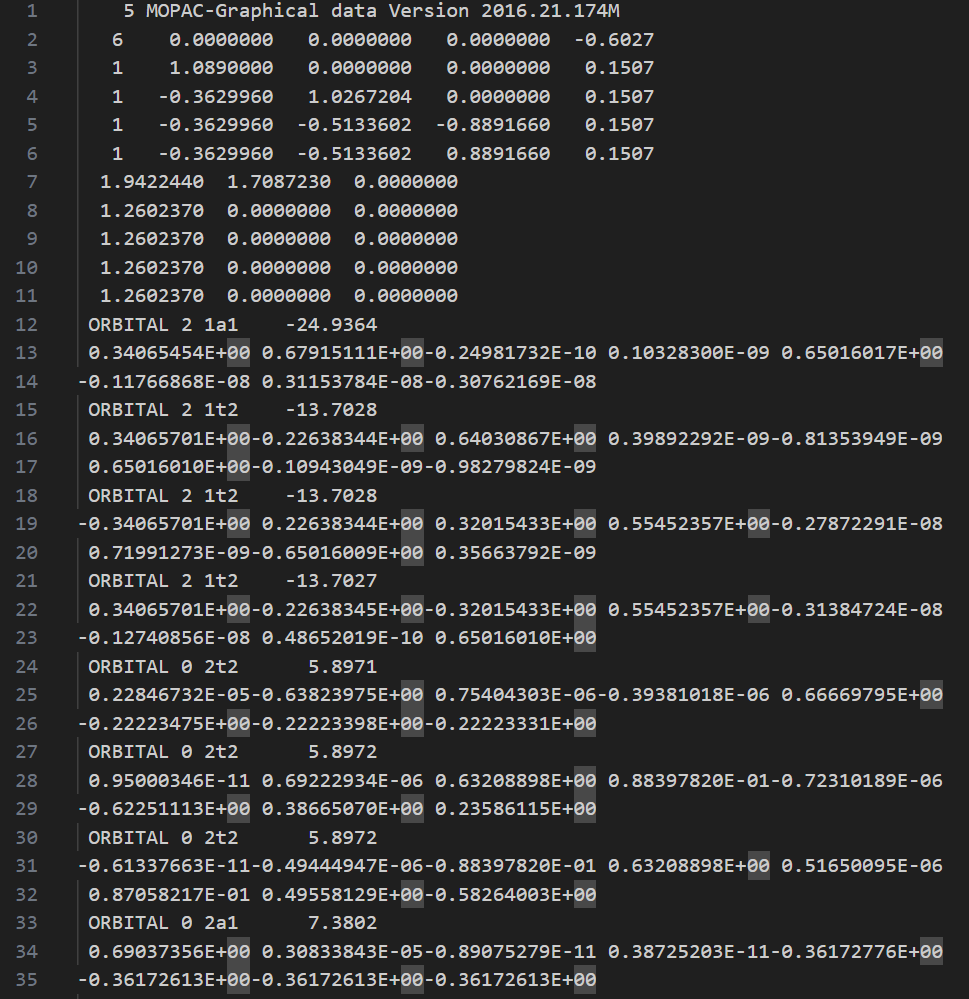
\includegraphics[width=\linewidth]{images autres/img_CH4-out_mgf.png}
    \caption{CH$_4$\_out.mgf}       
    \end{subfigure}
    \caption{Fichiers Entrée et Sortie MGF pour CH$_4$}
    \label{fig:placeholder}
\end{figure}

\begin{figure}[H]
    \centering
    \begin{subfigure}{0.49\textwidth}
    \centering
    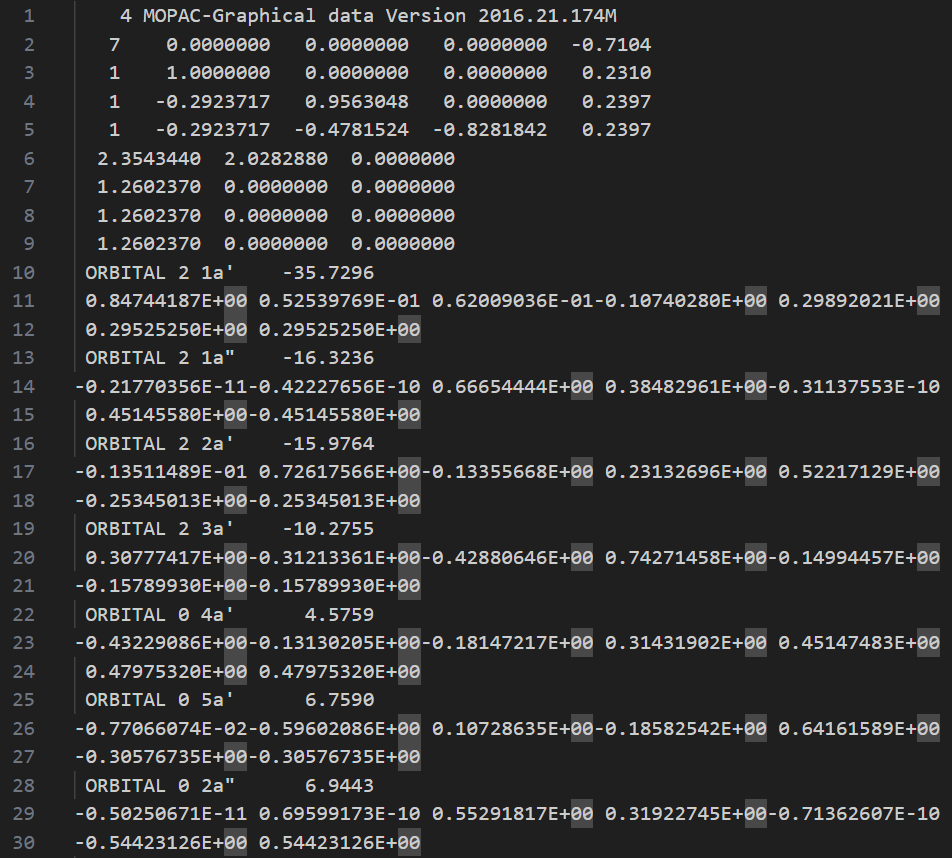
\includegraphics[width=\linewidth]{images autres/img_NH3_mgf.png}
    \caption{NH$_3$.mgf}       
    \end{subfigure}
       \hspace{0.1cm}
    \begin{subfigure}{0.49\textwidth}
    \centering
    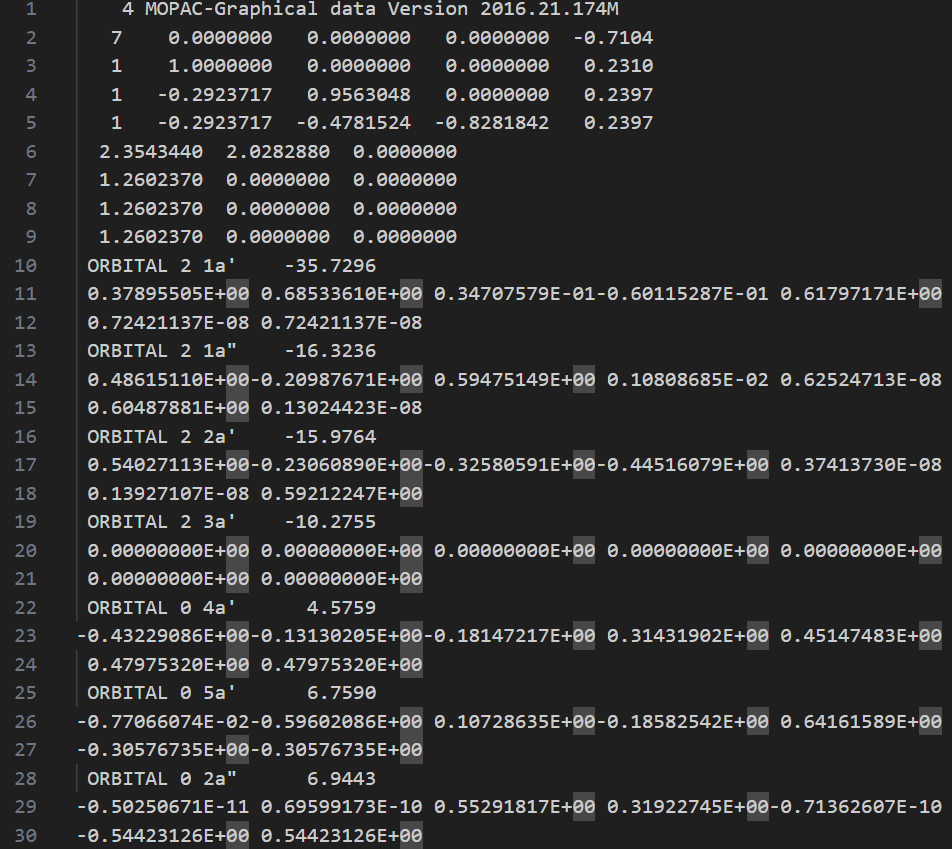
\includegraphics[width=\linewidth]{images autres/img_NH3-out_mgf.png}
    \caption{NH$_3$\_out.mgf}
    \end{subfigure}
    \caption{Fichiers Entrée et Sortie MGF pour NH$_3$}
    \label{fig:placeholder}
\end{figure}

\end{document}